% Options for packages loaded elsewhere
\PassOptionsToPackage{unicode}{hyperref}
\PassOptionsToPackage{hyphens}{url}
\PassOptionsToPackage{dvipsnames,svgnames,x11names}{xcolor}
%
\documentclass[
  letterpaper,
  DIV=11,
  numbers=noendperiod]{scrreprt}

\usepackage{amsmath,amssymb}
\usepackage{iftex}
\ifPDFTeX
  \usepackage[T1]{fontenc}
  \usepackage[utf8]{inputenc}
  \usepackage{textcomp} % provide euro and other symbols
\else % if luatex or xetex
  \usepackage{unicode-math}
  \defaultfontfeatures{Scale=MatchLowercase}
  \defaultfontfeatures[\rmfamily]{Ligatures=TeX,Scale=1}
\fi
\usepackage{lmodern}
\ifPDFTeX\else  
    % xetex/luatex font selection
\fi
% Use upquote if available, for straight quotes in verbatim environments
\IfFileExists{upquote.sty}{\usepackage{upquote}}{}
\IfFileExists{microtype.sty}{% use microtype if available
  \usepackage[]{microtype}
  \UseMicrotypeSet[protrusion]{basicmath} % disable protrusion for tt fonts
}{}
\makeatletter
\@ifundefined{KOMAClassName}{% if non-KOMA class
  \IfFileExists{parskip.sty}{%
    \usepackage{parskip}
  }{% else
    \setlength{\parindent}{0pt}
    \setlength{\parskip}{6pt plus 2pt minus 1pt}}
}{% if KOMA class
  \KOMAoptions{parskip=half}}
\makeatother
\usepackage{xcolor}
\usepackage{svg}
\setlength{\emergencystretch}{3em} % prevent overfull lines
\setcounter{secnumdepth}{5}
% Make \paragraph and \subparagraph free-standing
\ifx\paragraph\undefined\else
  \let\oldparagraph\paragraph
  \renewcommand{\paragraph}[1]{\oldparagraph{#1}\mbox{}}
\fi
\ifx\subparagraph\undefined\else
  \let\oldsubparagraph\subparagraph
  \renewcommand{\subparagraph}[1]{\oldsubparagraph{#1}\mbox{}}
\fi

\usepackage{color}
\usepackage{fancyvrb}
\newcommand{\VerbBar}{|}
\newcommand{\VERB}{\Verb[commandchars=\\\{\}]}
\DefineVerbatimEnvironment{Highlighting}{Verbatim}{commandchars=\\\{\}}
% Add ',fontsize=\small' for more characters per line
\usepackage{framed}
\definecolor{shadecolor}{RGB}{241,243,245}
\newenvironment{Shaded}{\begin{snugshade}}{\end{snugshade}}
\newcommand{\AlertTok}[1]{\textcolor[rgb]{0.68,0.00,0.00}{#1}}
\newcommand{\AnnotationTok}[1]{\textcolor[rgb]{0.37,0.37,0.37}{#1}}
\newcommand{\AttributeTok}[1]{\textcolor[rgb]{0.40,0.45,0.13}{#1}}
\newcommand{\BaseNTok}[1]{\textcolor[rgb]{0.68,0.00,0.00}{#1}}
\newcommand{\BuiltInTok}[1]{\textcolor[rgb]{0.00,0.23,0.31}{#1}}
\newcommand{\CharTok}[1]{\textcolor[rgb]{0.13,0.47,0.30}{#1}}
\newcommand{\CommentTok}[1]{\textcolor[rgb]{0.37,0.37,0.37}{#1}}
\newcommand{\CommentVarTok}[1]{\textcolor[rgb]{0.37,0.37,0.37}{\textit{#1}}}
\newcommand{\ConstantTok}[1]{\textcolor[rgb]{0.56,0.35,0.01}{#1}}
\newcommand{\ControlFlowTok}[1]{\textcolor[rgb]{0.00,0.23,0.31}{#1}}
\newcommand{\DataTypeTok}[1]{\textcolor[rgb]{0.68,0.00,0.00}{#1}}
\newcommand{\DecValTok}[1]{\textcolor[rgb]{0.68,0.00,0.00}{#1}}
\newcommand{\DocumentationTok}[1]{\textcolor[rgb]{0.37,0.37,0.37}{\textit{#1}}}
\newcommand{\ErrorTok}[1]{\textcolor[rgb]{0.68,0.00,0.00}{#1}}
\newcommand{\ExtensionTok}[1]{\textcolor[rgb]{0.00,0.23,0.31}{#1}}
\newcommand{\FloatTok}[1]{\textcolor[rgb]{0.68,0.00,0.00}{#1}}
\newcommand{\FunctionTok}[1]{\textcolor[rgb]{0.28,0.35,0.67}{#1}}
\newcommand{\ImportTok}[1]{\textcolor[rgb]{0.00,0.46,0.62}{#1}}
\newcommand{\InformationTok}[1]{\textcolor[rgb]{0.37,0.37,0.37}{#1}}
\newcommand{\KeywordTok}[1]{\textcolor[rgb]{0.00,0.23,0.31}{#1}}
\newcommand{\NormalTok}[1]{\textcolor[rgb]{0.00,0.23,0.31}{#1}}
\newcommand{\OperatorTok}[1]{\textcolor[rgb]{0.37,0.37,0.37}{#1}}
\newcommand{\OtherTok}[1]{\textcolor[rgb]{0.00,0.23,0.31}{#1}}
\newcommand{\PreprocessorTok}[1]{\textcolor[rgb]{0.68,0.00,0.00}{#1}}
\newcommand{\RegionMarkerTok}[1]{\textcolor[rgb]{0.00,0.23,0.31}{#1}}
\newcommand{\SpecialCharTok}[1]{\textcolor[rgb]{0.37,0.37,0.37}{#1}}
\newcommand{\SpecialStringTok}[1]{\textcolor[rgb]{0.13,0.47,0.30}{#1}}
\newcommand{\StringTok}[1]{\textcolor[rgb]{0.13,0.47,0.30}{#1}}
\newcommand{\VariableTok}[1]{\textcolor[rgb]{0.07,0.07,0.07}{#1}}
\newcommand{\VerbatimStringTok}[1]{\textcolor[rgb]{0.13,0.47,0.30}{#1}}
\newcommand{\WarningTok}[1]{\textcolor[rgb]{0.37,0.37,0.37}{\textit{#1}}}

\providecommand{\tightlist}{%
  \setlength{\itemsep}{0pt}\setlength{\parskip}{0pt}}\usepackage{longtable,booktabs,array}
\usepackage{calc} % for calculating minipage widths
% Correct order of tables after \paragraph or \subparagraph
\usepackage{etoolbox}
\makeatletter
\patchcmd\longtable{\par}{\if@noskipsec\mbox{}\fi\par}{}{}
\makeatother
% Allow footnotes in longtable head/foot
\IfFileExists{footnotehyper.sty}{\usepackage{footnotehyper}}{\usepackage{footnote}}
\makesavenoteenv{longtable}
\usepackage{graphicx}
\makeatletter
\def\maxwidth{\ifdim\Gin@nat@width>\linewidth\linewidth\else\Gin@nat@width\fi}
\def\maxheight{\ifdim\Gin@nat@height>\textheight\textheight\else\Gin@nat@height\fi}
\makeatother
% Scale images if necessary, so that they will not overflow the page
% margins by default, and it is still possible to overwrite the defaults
% using explicit options in \includegraphics[width, height, ...]{}
\setkeys{Gin}{width=\maxwidth,height=\maxheight,keepaspectratio}
% Set default figure placement to htbp
\makeatletter
\def\fps@figure{htbp}
\makeatother
% definitions for citeproc citations
\NewDocumentCommand\citeproctext{}{}
\NewDocumentCommand\citeproc{mm}{%
  \begingroup\def\citeproctext{#2}\cite{#1}\endgroup}
\makeatletter
 % allow citations to break across lines
 \let\@cite@ofmt\@firstofone
 % avoid brackets around text for \cite:
 \def\@biblabel#1{}
 \def\@cite#1#2{{#1\if@tempswa , #2\fi}}
\makeatother
\newlength{\cslhangindent}
\setlength{\cslhangindent}{1.5em}
\newlength{\csllabelwidth}
\setlength{\csllabelwidth}{3em}
\newenvironment{CSLReferences}[2] % #1 hanging-indent, #2 entry-spacing
 {\begin{list}{}{%
  \setlength{\itemindent}{0pt}
  \setlength{\leftmargin}{0pt}
  \setlength{\parsep}{0pt}
  % turn on hanging indent if param 1 is 1
  \ifodd #1
   \setlength{\leftmargin}{\cslhangindent}
   \setlength{\itemindent}{-1\cslhangindent}
  \fi
  % set entry spacing
  \setlength{\itemsep}{#2\baselineskip}}}
 {\end{list}}
\usepackage{calc}
\newcommand{\CSLBlock}[1]{\hfill\break\parbox[t]{\linewidth}{\strut\ignorespaces#1\strut}}
\newcommand{\CSLLeftMargin}[1]{\parbox[t]{\csllabelwidth}{\strut#1\strut}}
\newcommand{\CSLRightInline}[1]{\parbox[t]{\linewidth - \csllabelwidth}{\strut#1\strut}}
\newcommand{\CSLIndent}[1]{\hspace{\cslhangindent}#1}

\KOMAoption{captions}{tableheading}
\makeatletter
\@ifpackageloaded{tcolorbox}{}{\usepackage[skins,breakable]{tcolorbox}}
\@ifpackageloaded{fontawesome5}{}{\usepackage{fontawesome5}}
\definecolor{quarto-callout-color}{HTML}{909090}
\definecolor{quarto-callout-note-color}{HTML}{0758E5}
\definecolor{quarto-callout-important-color}{HTML}{CC1914}
\definecolor{quarto-callout-warning-color}{HTML}{EB9113}
\definecolor{quarto-callout-tip-color}{HTML}{00A047}
\definecolor{quarto-callout-caution-color}{HTML}{FC5300}
\definecolor{quarto-callout-color-frame}{HTML}{acacac}
\definecolor{quarto-callout-note-color-frame}{HTML}{4582ec}
\definecolor{quarto-callout-important-color-frame}{HTML}{d9534f}
\definecolor{quarto-callout-warning-color-frame}{HTML}{f0ad4e}
\definecolor{quarto-callout-tip-color-frame}{HTML}{02b875}
\definecolor{quarto-callout-caution-color-frame}{HTML}{fd7e14}
\makeatother
\makeatletter
\@ifpackageloaded{bookmark}{}{\usepackage{bookmark}}
\makeatother
\makeatletter
\@ifpackageloaded{caption}{}{\usepackage{caption}}
\AtBeginDocument{%
\ifdefined\contentsname
  \renewcommand*\contentsname{Table of contents}
\else
  \newcommand\contentsname{Table of contents}
\fi
\ifdefined\listfigurename
  \renewcommand*\listfigurename{List of Figures}
\else
  \newcommand\listfigurename{List of Figures}
\fi
\ifdefined\listtablename
  \renewcommand*\listtablename{List of Tables}
\else
  \newcommand\listtablename{List of Tables}
\fi
\ifdefined\figurename
  \renewcommand*\figurename{Figure}
\else
  \newcommand\figurename{Figure}
\fi
\ifdefined\tablename
  \renewcommand*\tablename{Table}
\else
  \newcommand\tablename{Table}
\fi
}
\@ifpackageloaded{float}{}{\usepackage{float}}
\floatstyle{ruled}
\@ifundefined{c@chapter}{\newfloat{codelisting}{h}{lop}}{\newfloat{codelisting}{h}{lop}[chapter]}
\floatname{codelisting}{Listing}
\newcommand*\listoflistings{\listof{codelisting}{List of Listings}}
\makeatother
\makeatletter
\makeatother
\makeatletter
\@ifpackageloaded{caption}{}{\usepackage{caption}}
\@ifpackageloaded{subcaption}{}{\usepackage{subcaption}}
\makeatother
\ifLuaTeX
  \usepackage{selnolig}  % disable illegal ligatures
\fi
\usepackage{bookmark}

\IfFileExists{xurl.sty}{\usepackage{xurl}}{} % add URL line breaks if available
\urlstyle{same} % disable monospaced font for URLs
\hypersetup{
  pdftitle={Open Soil Spectral Library},
  pdfauthor={Soil Spectroscopy for Global Good team},
  colorlinks=true,
  linkcolor={blue},
  filecolor={Maroon},
  citecolor={Blue},
  urlcolor={Blue},
  pdfcreator={LaTeX via pandoc}}

\title{Open Soil Spectral Library}
\author{Soil Spectroscopy for Global Good team}
\date{2026-03-15}

\begin{document}
\maketitle

\renewcommand*\contentsname{Table of contents}
{
\hypersetup{linkcolor=}
\setcounter{tocdepth}{2}
\tableofcontents
}
\bookmarksetup{startatroot}

\chapter*{Welcome!}\label{welcome}
\addcontentsline{toc}{chapter}{Welcome!}

\markboth{Welcome!}{Welcome!}

\href{https://github.com/soilspectroscopy}{\includegraphics{index_files/mediabag/github--121011.svg-style=for-the-badge-logo=github-log}}

\href{https://doi.org/10.5281/zenodo.5759693}{\includesvg{index_files/mediabag/zenodo.5759693.svg}}

Welcome to the Open Soil Spectral Library (OSSL) manual!

The OSSL is a public and growing dataset that is compiled by the
\href{https://soilspectroscopy.org/}{Soil Spectroscopy for Global Good}
initiative.

A \href{https://doi.org/10.1371/journal.pone.0296545}{peer-reviewed and
open-access publication} is available for additional reference.

Please navigate to the different sections to learn more about:

\begin{itemize}
\tightlist
\item
  📘 \hyperref[sec-about]{About}: Our team, OSSL resources,
  contributors, citation, and other information.
\item
  📘 \hyperref[sec-soilspec]{Soil Spectroscopy}: Soil spectroscopy in
  general, predictive modeling, imported soil spectral libraries,
  instruments and software.
\item
  📘 \hyperref[sec-db-desc]{Database description}: Database definitions,
  including variable names, types, human-readable description, and
  example values.
\item
  📘 \hyperref[sec-db-access]{Database access}: Ways of accessing the
  OSSL.
\item
  📘 \hyperref[sec-neospectra]{Neospectra database}: Data, models, and
  studies from a low-cost NIR scanner.
\item
  📘 \hyperref[sec-prediction-models]{Predictive models}: Fitted models
  with the OSSL.
\item
  📘 \hyperref[sec-web-services]{Web services}: User-friendly and online
  applications.
\item
  📘 \hyperref[sec-tutorial]{Hands-on tutorial}: Training materials.
\item
  📘 \hyperref[sec-publications]{Scientific publications}: Papers that
  our team or collaborators have published.
\item
  📘 \hyperref[sec-references]{References}.
\end{itemize}

\bookmarksetup{startatroot}

\chapter*{About}\label{sec-about}
\addcontentsline{toc}{chapter}{About}

\markboth{About}{About}

\begin{quote}
``Man's most human characteristic is not his ability to learn, which he
shares with many other species, but his ability to teach and store what
others have developed and taught him.'' Margaret Mead, Culture and
Commitment: The New Relationships Between the Generations in the 1970s.
\end{quote}

\section*{Soil Spectroscopy for Global
Good}\label{soil-spectroscopy-for-global-good}
\addcontentsline{toc}{section}{Soil Spectroscopy for Global Good}

\markright{Soil Spectroscopy for Global Good}

The SS4GG was created by
\href{https://www.woodwellclimate.org/}{Woodwell Climate Research
Center}, \href{https://opengeohub.org/}{OpenGeoHub Foundation}, and
\href{https://www.essie.ufl.edu/}{University of Florida}, and was
formally funded by the USDA National Institute of Food and Agriculture
(NIFA) Cyberinformatics Tools Coordinated Innovation Network, award
\href{https://portal.nifa.usda.gov/web/crisprojectpages/1023775-fact-cin-soil-spectroscopy-for-the-global-good.html}{2020-67021-32467}
between 2021 and 2024. It brought together soil scientists, data
scientists and other stakeholders to overcome some of the current
bottlenecks preventing a wider and more efficient use of soil
spectroscopy. A series of activities addressed many topics including
interoperability, machine learning, community events, and application of
spectroscopy predictions for informed decision-making. For more
information about the initiative, please refer to our
\href{https://soilspectroscopy.org/}{official webpage}.

\href{https://soilspectroscopy.org/}{\begin{center}
\includegraphics[width=0.5\textwidth,height=\textheight]{img/soilspec4gg-logo_fc.png}
\end{center}
}

As the original project has ended, SS4GG keeps running and improving its
resources with funding from
\href{https://www.woodwellclimate.org/air-quality-monitoring-to-machine-learning-fund-for-climate-solutions-awards-six-new-grants/}{Woodwell
Climate}, \href{https://opengeohub.org/}{OpenGeoHub}, and
\href{https://www.llnl.gov/article/50411/lawrence-livermore-grabs-two-spots-does-energy-earthshot-program}{Department
of Energy's (DOE)}, while working to secure a new round of multiyear
funding.

SS4GG also works with other global initiatives including the
\href{https://www.fao.org/global-soil-partnership/glosolan-old/soil-analysis/dry-chemistry-spectroscopy/en/}{FAO
Global Soil Partnership} and the
\href{https://sagroups.ieee.org/4005/}{IEEE P4005 - Standards and
Protocols for Soil Spectroscopy} working group.

\section*{Open Soil Spectral Library}\label{open-soil-spectral-library}
\addcontentsline{toc}{section}{Open Soil Spectral Library}

\markright{Open Soil Spectral Library}

The Open Soil Spectral Library (OSSL) is a compilation of several
heterogenous and independent datasets into a common standardized source.
It is available as a digital asset and web-services. The OSSL
compilation allowed our team to fit generally-applicable prediction
models based on spectral measurements. Several resources are built
around the OSSL, which includes:

\begin{itemize}
\tightlist
\item
  A public soil spectral library shared through several formats
  \href{https://soilspectroscopy.github.io/ossl-manual/database-access.html}{(S3,
  mongoDB, and API)} and
  \href{https://soilspectroscopy.github.io/ossl-manual/database-description.html}{documented}
  in this manual;
\item
  \href{https://api.soilspectroscopy.org/__docs__/\#/}{API} with
  database access and an estimation service;
\item
  Web services facilitating user interaction:
  \href{https://explorer.soilspectroscopy.org/}{OSSL Explorer} and
  \href{https://engine.soilspectroscopy.org/}{OSSL Engine};
\item
  \href{https://github.com/soilspectroscopy}{Open-source code on GitHub}
  used for data compilation, analysis, and machine learning;
\item
  \href{https://soilspectroscopy.github.io/ossl-manual/hands-on-tutorial.html}{Tutorials
  and training materials}.
\end{itemize}

\begin{tcolorbox}[enhanced jigsaw, title=\textcolor{quarto-callout-tip-color}{\faLightbulb}\hspace{0.5em}{Publication alert!}, rightrule=.15mm, coltitle=black, opacityback=0, bottomrule=.15mm, colframe=quarto-callout-tip-color-frame, breakable, arc=.35mm, titlerule=0mm, toptitle=1mm, left=2mm, colback=white, toprule=.15mm, leftrule=.75mm, bottomtitle=1mm, opacitybacktitle=0.6, colbacktitle=quarto-callout-tip-color!10!white]

A peer-reviewed and open-access publication describing the first version
of OSSL database and initial predictive modeling is available in
\href{https://doi.org/10.1371/journal.pone.0296545}{PLOS One}. Please
use the following info when citing the OSSL:

\begin{quote}
Safanelli, J. L., Hengl, T., Parente, L. L., Minarik, R., Bloom, D. E.,
Todd-Brown, K., \ldots{} Sanderman, J. (2025). Open Soil Spectral
Library (OSSL): Building reproducible soil calibration models through
open development and community engagement. PloS One, 20(1), e0296545.
doi:\href{https://doi.org/10.1371/journal.pone.0296545}{10.1371/journal.pone.0296545}.
\end{quote}

\end{tcolorbox}

\section*{Contributors}\label{contributors}
\addcontentsline{toc}{section}{Contributors}

\markright{Contributors}

Over the past years several people have contributed or are still
contributing with the SS4GG. The following list is not exhaustive:

\begin{itemize}
\tightlist
\item
  José Lucas Safanelli (core team)
\item
  Ran Zhi (core team)
\item
  Tomislav Hengl (core team)
\item
  Jonathan Sanderman (core team)
\item
  Katherine Todd-Brown (core team)
\item
  Rich Ferguson (advisory board)
\item
  Fenny van Egmond (advisory board)
\item
  Keith Shepherd (advisory board)
\item
  Leandro Parente (dev and project contributor)
\item
  Robert Minarik (project contributor)
\item
  Dellena E. Bloom (project contributor)
\item
  Wanderson de Sousa Mendes (project contributor)
\item
  Asa Gholizadeh (project contributor)
\item
  Colleen Partida (project contributor)
\item
  Aleksandar Sekulic (web services)
\item
  Petar Bursac (web services)
\item
  Henning Teickner (github contributor)
\item
  Deepak C. (github contributor)
\item
  Philipp Baumann (foss dev and github contributor)
\item
  Franck Albinet (foss dev)
\item
  Laura Summerauer (data contributor)
\item
  Marcus Schiedung (data contributor)
\item
  Loretta Garrett (data contributor)
\item
  Branislav Jović (data contributor)
\end{itemize}

\section*{Acknowledgments}\label{acknowledgments}
\addcontentsline{toc}{section}{Acknowledgments}

\markright{Acknowledgments}

\begin{tcolorbox}[enhanced jigsaw, title=\textcolor{quarto-callout-tip-color}{\faLightbulb}\hspace{0.5em}{Funding}, rightrule=.15mm, coltitle=black, opacityback=0, bottomrule=.15mm, colframe=quarto-callout-tip-color-frame, breakable, arc=.35mm, titlerule=0mm, toptitle=1mm, left=2mm, colback=white, toprule=.15mm, leftrule=.75mm, bottomtitle=1mm, opacitybacktitle=0.6, colbacktitle=quarto-callout-tip-color!10!white]

Soil Spectroscopy for Global Good (SS4GG) was formally funded by USDA
NIFA Award
\href{https://portal.nifa.usda.gov/web/crisprojectpages/1023775-fact-cin-soil-spectroscopy-for-the-global-good.html}{2020-67021-32467}
between 2021-2024. It has been currently and partially supported by
Woodwell Climate, OpenGeoHub, and the US Department of Energy.

\end{tcolorbox}

\begin{itemize}
\tightlist
\item
  \href{https://ncsslabdatamart.sc.egov.usda.gov/}{\textbf{USDA-NRCS
  Kellogg Soil Survey Laboratory (KSSL)}}, especially Rich Ferguson,
  Scarlett Murphy, Skye Wills, and Jonathan Maynard, for hosting the
  KSSL MIR {[}1{]} and RaCA VisNIR {[}2{]} databases in the public
  domain, while assisting and answering many questions about the
  databases and laboratory SOPs;
\item
  \href{https://www.cifor-icraf.org/}{\textbf{World Agroforestry ICRAF}}
  \&
  \href{https://www.isric.org/explore/isric-soil-data-hub}{\textbf{World
  Soil Information ISRIC}} for releasing a VisNIR soil spectral library
  {[}3{]} based on the Soil Information System (ISIS) of ISRIC;
\item
  \href{https://www.cifor-icraf.org/}{\textbf{World Agroforestry
  (ICRAF)}} for releasing the
  \href{https://data.worldagroforestry.org/dataverse/icraf_soils}{Africa
  Soil Information Service (AfSIS)} phases I and II MIR spectral
  libraries {[}4{]}, a collaborative project funded by the Bill and
  Melinda Gates Foundation (BMGF). Partners included: CIAT-TSBF, ISRIC,
  CIESIN, The Earth Institute at Columbia University and World
  Agroforestry (ICRAF);
\item
  \href{http://esdac.jrc.ec.europa.eu/}{\textbf{European Soil Data
  Centre}} for making openly available the LUCAS Soil Spectral Library
  {[}5{]}.;
\item
  Laura Summerauer from \textbf{ETH Zurich}, for sharing the Central
  African Soil Spectral Library {[}6{]};
\item
  Marcus Schiedung (formerly from \textbf{University of Zurich}, now
  \textbf{Thünen Institute}) for sharing a MIR soil spectral library
  from forest soils of North Canada {[}7{]};
\item
  Loretta Garrett from \textbf{Scion Research} for sharing several MIR
  spectral datasets from forest soils in New Zealand {[}8{]};
\item
  Branislav Jović from the \textbf{University of Novi Sad} for sharing a
  MIR soil spectral library from Serbian soils {[}9{]};
\end{itemize}

\section*{Disclaimer}\label{disclaimer}
\addcontentsline{toc}{section}{Disclaimer}

\markright{Disclaimer}

Whilst utmost care has been taken by the Soil Spectroscopy project and
data authors while collecting and compiling the data, the data is
provided ``as is''. Woodwell Climate Research Center, University of
Florida, OpenGeoHub foundation and its suppliers and licensors hereby
disclaim all warranties of any kind, express or implied, including,
without limitation, the warranties of merchantability, fitness for a
particular purpose and non-infringement. Neither Woodwell Climate
Research Center, University of Florida, OpenGeoHub foundation nor its
suppliers and licensors, makes any warranty that the Website will be
error free or that access thereto will be continuous or uninterrupted.
You understand that you download from, or otherwise obtain content or
services through, the Website at your own discretion and risk.

In no event shall the data authors, the Soil Spectroscopy project, or
relevant funding agencies be liable for any actual, incidental or
consequential damages arising from use of the data. By using the Soil
Spectroscopy project data, the user expressly acknowledges that the Data
may contain some nonconformities, defects, or errors. No warranty is
given that the data will meet the user's needs or expectations or that
all nonconformities, defects, or errors can or will be corrected. The
user should always verify actual data; therefore the user bears all
responsibility in determining whether the data is fit for the user's
intended use.

The data and manual is always under improvement. If you notice an error
or outdated information, please submit a correction/pull request to our
github repository or send us an email!

This is a community project. No profits are being made from building and
serving the Open Soil Spectral Library.

\section*{License}\label{license}
\addcontentsline{toc}{section}{License}

\markright{License}

This manual and all project code is free to use, and if not otherwise
indicated, is licensed under the MIT License. The OSSL training data and
models, if not otherwise indicated, are available under the Creative
Commons Attribution 4.0 International CC-BY.

\section*{How to cite}\label{how-to-cite}
\addcontentsline{toc}{section}{How to cite}

\markright{How to cite}

We highly recommend citing the OSSL paper for everything related to the
OSSL and SS4GG initiative:

\begin{verbatim}
@article{Safanelli2025,
  title    = "Open Soil Spectral Library ({OSSL)}: Building reproducible soil
              calibration models through open development and community
              engagement",
  author   = "Safanelli, Jos{\'e} L and Hengl, Tomislav and Parente, Leandro L
              and Minarik, Robert and Bloom, Dellena E and Todd-Brown,
              Katherine and Gholizadeh, Asa and Mendes, Wanderson de Sousa and
              Sanderman, Jonathan",
  journal  = "PLoS One",
  volume   =  20,
  number   =  1,
  pages    = "e0296545",
  month    =  jan,
  year     =  2025,
  language = "en",
  doi = {10.1371/journal.pone.0296545}
}
\end{verbatim}

If otherwise you just want to cite the manual, please use the following:

\begin{verbatim}
@misc{OSSL_manual,
  author = {Soil Spectroscopy for Global Good team},
  title = {Open Soil Spectral Library Manual},
  year = 2025,
  url = {https://soilspectroscopy.github.io/ossl-manual/},
  doi = {https://doi.org/10.5281/zenodo.5759693},
  urldate = {2025-01-13}
}
\end{verbatim}

\bookmarksetup{startatroot}

\chapter{Soil spectroscopy}\label{sec-soilspec}

\section{What is soil spectroscopy}\label{what-is-soil-spectroscopy}

Soil spectroscopy refers to the measurement of light interaction with
soil. Various methods exist to measure this interaction with the goal of
understanding the mineral and organic composition of soils. The most
common technique is to measure the absorption when a non-collimated flux
of light from the
\href{https://en.wikipedia.org/wiki/Electromagnetic_spectrum}{visible
and infrared region of the electromagnetic spectrum} is applied to a
soil surface. The proportion of the incident radiation reflected by the
soil compared to a reference material is measured, forming the basis of
\href{https://en.wikipedia.org/wiki/Diffuse_reflectance_spectroscopy}{diffuse
reflectance spectroscopy}. Distinct characteristic spectra can then be
used to estimate various soil properties, including particle size
distribution, minerals, and organic compounds. The OSSL is composed of
diffuse reflectance spectra collected across the visible (Vis), near-
(NIR), and mid-infrared (MIR) regions.

\begin{tcolorbox}[enhanced jigsaw, title=\textcolor{quarto-callout-tip-color}{\faLightbulb}\hspace{0.5em}{Spectral regions}, rightrule=.15mm, coltitle=black, opacityback=0, bottomrule=.15mm, colframe=quarto-callout-tip-color-frame, breakable, arc=.35mm, titlerule=0mm, toptitle=1mm, left=2mm, colback=white, toprule=.15mm, leftrule=.75mm, bottomtitle=1mm, opacitybacktitle=0.6, colbacktitle=quarto-callout-tip-color!10!white]

Visible and near-infrared (VisNIR) is typically represented between
350--2500 nm, while the mid-infrared (MIR) ranges between 2500--25000 nm
(formally described as 4000--400 cm\textsuperscript{-1}). In the OSSL,
we have also imported a specific near-infrared library built with the
Neospectra scanner (Si-Ware), with its range covering the 1350-2550 nm
region.

\end{tcolorbox}

\begin{figure}[H]

{\centering \includegraphics{img/drs-schematic.jpeg}

}

\caption{Schematic explanation of diffuse reflectance spectroscopy for
soil analysis.}

\end{figure}%

With a collection of soil spectra and corresponding soil properties
measured by conventional methods, one can fit
\href{https://soilspectroscopy.github.io/soilspec-workshop/intro.html}{predictive
models} to quantitatively estimate various soil properties on new
scanned soil samples. This method is cost-effective, faster, does not
produce chemical residues, and is more scalable than traditional soil
analysis techniques. A soil spectral library, such as the OSSL, provides
the training data for building and testing predictive models, which are
typically developed using machine learning or chemometric algorithms.
The effectiveness of these predictive models depends significantly on
how well the library represents the variability and diversity of both
current and new soil samples intended for prediction.

\section{Estimating soil properties}\label{estimating-soil-properties}

Given that each soil spectral library that was imported into the OSSL
used distinct procedures for analytically determining reference values,
the incompatibility has been a subject of internal discussion in this
project. Some global initiatives have been facing this same issue in
their soil databases but there still no clear or full consensus on how
to harmonize those different methods. This has been a topic of great
discussion and research development at the
\href{https://www.fao.org/global-soil-partnership/glosolan/en/}{Global
Soil Partnership's Global Soil Laboratory Network (GLOSOLAN)}.

In order to maximize transparency, for now, we have decided to produce
two different levels for the OSSL database. \texttt{Level\ 0} takes into
account the original methods employed in each dataset but tries to
initially fit them to two reference lists:
\href{https://www.nrcs.usda.gov/resources/guides-and-instructions/kssl-guidance}{KSSL
Guidance -- Laboratory Methods and Manuals} and ISO standards. A copy of
the KSSL procedures and coding scheme is archived in
\href{https://github.com/soilspectroscopy/ossl-imports/blob/main/out/kssl_procedures.csv}{ossl-imports}.

If a reference method does not fall in any previous method, then we
create a new variable sharing at least a common property and unit. A
final harmonization takes place in the OSSL \texttt{Level\ 1}, where
those common properties sharing different methods are converted to a
target method using some publicly available transformation rule, or in
the worst scenario, they are naively binded or kept separated to produce
its specific model. All the implementations are documented in the
\href{https://github.com/soilspectroscopy/ossl-imports/blob/main/out/ossl_level0_to_level1_soillab_harmonization.csv}{ossl-import/ossl\_level0\_to\_level1\_soillab\_harmonization.csv}
repository.

In addition,
\href{http://www.fao.org/global-soil-partnership/glosolan/soil-analysis}{GLOSOLAN's
Standard Operating Procedures (SOPs)} list four groups of soil variables
of interest to international soil spectroscopy projects:

Soil chemical variables:

\begin{itemize}
\tightlist
\item
  pH,\\
\item
  Carbon,\\
\item
  Phosphorous,\\
\item
  Potassium,\\
\item
  Nitrogen,\\
\item
  Exchangeable cations and CEC,\\
\item
  Extractable microelements,\\
\item
  Trace and major element analyses,\\
\item
  Gypsum,\\
\item
  Electrical conductivity and total soluble salt content,\\
\item
  Soluble sulfate and chloride analysis,\\
\item
  Special analysis for peats, mineral and organic soils, agriculture and
  forest.
\end{itemize}

Soil physical variables:

\begin{itemize}
\tightlist
\item
  Bulk density,\\
\item
  Coarse fragments,\\
\item
  Particle-size distribution,\\
\item
  Water retention curve,\\
\item
  Porosity,\\
\item
  Hydraulic conductivity function,\\
\item
  Aggregate stability,\\
\item
  Moisture content,
\end{itemize}

Soil biological variables:

\begin{itemize}
\tightlist
\item
  Microbial biomass,\\
\item
  Soil Respiration,\\
\item
  Enzyme activity,\\
\item
  Microbial identification,
\end{itemize}

Soil contaminants:

\begin{itemize}
\tightlist
\item
  Heavy metal elements: As, Hg, Cu, Cd, Pb and similar,\\
\item
  Other soil pollutants,
\end{itemize}

\section{Predictive modeling}\label{predictive-modeling}

From initial findings with the OSSL {[}10{]}, on average, the MIR range
appears to be the best spectral region for developing spectral
prediction models, followed by VisNIR and NIR (Neospectra). This happens
because the MIR contains several fundamental and resolved absorption
features from mineral and organic functional groups that translate to
better prediction capacity, despite challenges in the interpretation
that stem from chemical heterogeneity. VisNIR and NIR spectra, in turn,
are made of overtones from the fundamental vibrations of the MIR range,
hence, are less sensitive to soil constituents and may result in
inferior performance. In addition, we found good performance for some
soil properties that may not directly affect soil spectra but can be
indirectly inferred and quantified (secondary properties), such as
cation exchange capacity, pH, soil contaminants, etc. However,
understanding both primary and secondary components in the soil helps to
better understand the factors that contribute to the improvement of
spectral predictive models within the complex context of soil systems
and also to select the spectral range, where they are most pronounced.

\begin{figure}[H]

{\centering \includegraphics{img/fig5-pone-ossl.PNG}

}

\caption{\textbf{Rank of prediction models fitted with the Open Soil
Spectral Library (OSSL)}. Lin's concordance correlation coefficient
(CCC) from 10-fold cross-validation with refitting. Striped bars
represent models with a ratio of performance to the interquartile range
(RPIQ) \textless{} 2. Source: {[}10{]}}

\end{figure}%

We recommend visiting a
\href{https://soilspectroscopy.github.io/soilspec-workshop/}{\textbf{dedicated
tutorial}} where we present and walk through the modeling framework
employed with the OSSL. We recommend checking the introduction section
to understand why soil spectroscopy is a \textbf{fit-for-purpose
technology}, why \textbf{good predictions flow only from good data}, and
the \textbf{best practices for model calibration}.

The OSSL paper {[}10{]} also describes and validates in detail the OSSL
models.

\section{Instruments}\label{instruments}

A
\href{https://openknowledge.fao.org/items/43aca83e-f3eb-4648-9f61-e3acdc7e62a3}{Global
Soil Spectroscopy Assessment} was published in 2021 by FAO {[}11{]},
where a number of instruments were identified in soil spectroscopy
laboratories. Within the SS4GG initiative, we published a paper on the
spectral dissimilarity of 20 MIR instruments {[}12{]} providing clear
recommendations to overcome this problem. A second analysis of VisNIR
instruments is being developed in collaboration with the
\href{https://sagroups.ieee.org/4005/}{IEEE P4005 working group}.

\begin{figure}[H]

{\centering \includegraphics{img/ssl_instruments_list.png}

}

\caption{Most frequent MIR and VisNIR instruments reported in {[}11{]}}

\end{figure}%

\section{Software}\label{software}

There are many proprietary and open source software used to process
spectral measurements. We provide below a list (not exhaustive) of the
most common packages/modules that can be used in R or Python (both FOSS)
for importing, preprocessing, and analyzing soil spectral data:

\subsection{SoilSpecData}\label{soilspecdata}

\begin{itemize}
\tightlist
\item
  📛 Name: SoilSpecData\\
\item
  💼 Specialty: A Python package for handling soil spectroscopy data,
  with a focus on the Open Soil Spectral Library (OSSL) in Python.\\
\item
  💻 Programming language: Python\\
\item
  🔗 Homepage: \href{https://fr.anckalbi.net/soilspecdata/}{Website},
  \href{https://github.com/franckalbinet/soilspecdata}{GitHub}\\
\item
  📕 Albinet, F. SoilSpecData: A Python package for handling soil
  spectroscopy data, with a focus on the Open Soil Spectral Library
  (OSSL). Python package. Available in:
  \url{https://fr.anckalbi.net/soilspecdata/}.\\
\item
  ©️ License:
  \href{https://github.com/franckalbinet/soilspecdata?tab=Apache-2.0-1-ov-file\#readme}{Apache-2.0
  license}
\item
  📧 Maintainer: \href{https://github.com/franckalbinet}{Franck Albinet}
\end{itemize}

\subsection{SoilSpecTfm}\label{soilspectfm}

\begin{itemize}
\tightlist
\item
  📛 Name: SoilSpecTfm\\
\item
  💼 Specialty: A Python package for handling soil spectroscopy data,
  with a focus on the Open Soil Spectral Library (OSSL) in Python.\\
\item
  💻 Programming language: Python\\
\item
  🔗 Homepage: \href{https://fr.anckalbi.net/soilspectfm/}{Website},
  \href{https://github.com/franckalbinet/soilspecdata}{GitHub}\\
\item
  📕 Albinet, F. SoilSpecTfm: Provides Scikit-Learn compatible
  transforms for spectroscopic data preprocessing. Python package.
  Available in: \url{https://github.com/franckalbinet/soilspectfm}.\\
\item
  ©️ License:
  \href{https://github.com/franckalbinet/soilspectfm\#Apache-2.0-1-ov-file}{Apache-2.0
  license}
\item
  📧 Maintainer: \href{https://github.com/franckalbinet}{Franck Albinet}
\end{itemize}

\subsection{opusreader2}\label{opusreader2}

\begin{itemize}
\tightlist
\item
  📛 Name: opusreader2\\
\item
  💼 Specialty: Read OPUS binary files from Fourier-Transform Infrared
  (FT-IR) spectrometers of the company Bruker Optics GmbH \& Co.~in R
\item
  💻 Programming language: R\\
\item
  🔗 Homepage:
  \href{https://github.com/spectral-cockpit/opusreader2}{GitHub}\\
\item
  📕 Baumann P, Knecht T, Roudier P (2023). opusreader2: Read
  spectroscopic data from Bruker OPUS binary Files. R package version
  0.6.3.\\
\item
  ©️ License:
  \href{https://github.com/spectral-cockpit/opusreader2/blob/main/LICENSE}{MIT}
\item
  📧 Maintainer:
  \href{https://github.com/spectral-cockpit}{spectral-cockpit}
\end{itemize}

\subsection{asdreader}\label{asdreader}

\begin{itemize}
\tightlist
\item
  📛 Name: asdreader
\item
  💼 Specialty: Reading ASD binary files in R\\
\item
  💻 Programming language: R\\
\item
  🔗 Homepage:
  \href{https://github.com/pierreroudier/asdreader}{GitHub}\\
\item
  📕 Roudier, P. (2020). asdreader: reading ASD binary files in R. R
  package version 0.1-3 CRAN.\\
\item
  ©️ License: GPL\\
\item
  📧 Maintainer: \href{https://github.com/pierreroudier}{Pierre Roudier}
\end{itemize}

\subsection{prospectr}\label{prospectr}

\begin{itemize}
\tightlist
\item
  📛 Name: prospectr\\
\item
  💼 Specialty: Signal processing, resampling\\
\item
  💻 Programming language: R\\
\item
  🔗 Homepage:
  \href{https://github.com/l-ramirez-lopez/prospectr}{GitHub}\\
\item
  📕 Stevens, A., \& Ramirez-Lopez, L. (2022). An introduction to the
  prospectr package. R Package Vignette. R Package Version 0.2.6.\\
\item
  ©️ License: \href{https://cran.r-project.org/web/licenses/MIT}{MIT} +
  \href{https://cran.r-project.org/web/packages/prospectr/LICENSE}{file
  LICENSE}\\
\item
  📧 Maintainer: \href{https://github.com/l-ramirez-lopez}{Leornardo
  Ramirez-Lopez}
\end{itemize}

\subsection{simplerspec}\label{simplerspec}

\begin{itemize}
\tightlist
\item
  📛 Name: simplerspec\\
\item
  💼 Specialty: Soil and plant spectroscopic model building and
  prediction\\
\item
  💻 Programming language: R\\
\item
  🔗 Homepage:
  \href{https://philipp-baumann.github.io/simplerspec}{GitHub}\\
\item
  📕 Baumann, P. (2020). simplerspec: Soil and plant spectroscopic model
  building and prediction. Packages R CRAN.\\
\item
  ©️ License:
  \href{https://github.com/philipp-baumann/simplerspec/blob/master/LICENSE.md}{GNU
  General Public License v3.0}\\
\item
  📧 Maintainer: \href{https://github.com/philipp-baumann}{Philipp
  Baumann}
\end{itemize}

\subsection{resemble}\label{resemble}

\begin{itemize}
\tightlist
\item
  📛 Name: resemble\\
\item
  💼 Specialty: Memory-based learning in spectral chemometrics
\item
  💻 Programming language: R\\
\item
  🔗 Homepage:
  \href{https://github.com/l-ramirez-lopez/resemble}{GitHub}\\
\item
  📕 Ramirez-Lopez, L., and Stevens, A., and Viscarra Rossel, R., and
  Lobsey, C., and Wadoux, A., and Breure, T. (2022). resemble:
  Regression and similarity evaluation for memory-based learning in
  spectral chemometrics. R package Vignette. R package version 2.2.1.
\item
  ©️ License: \href{https://cran.r-project.org/web/licenses/MIT}{MIT} +
  \href{https://github.com/l-ramirez-lopez/resemble/blob/main/LICENSE}{file
  LICENSE}
\item
  📧 Maintainer: \href{https://github.com/l-ramirez-lopez}{Leonardo
  Ramirez Lopez}
\end{itemize}

\subsection{mdatools}\label{mdatools}

\begin{itemize}
\tightlist
\item
  📛 Name: mdatools\\
\item
  💼 Specialty: A package for preprocessing, exploring and analysis of
  multivariate data. The package provides methods mostly common for
  Chemometrics.
\item
  💻 Programming language: R\\
\item
  🔗 Homepage: \href{https://www.mdatools.com/}{Website},
  \href{https://github.com/svkucheryavski/mdatools}{GitHub}\\
\item
  📕 Kucheryavskiy, S. (2020). mdatools -- R package for chemometrics.
  Chemometrics and Intelligent Laboratory Systems: An International
  Journal Sponsored by the Chemometrics Society, 198(103937), 103937.
  doi:\href{https://doi.org/10.1016/j.chemolab.2020.103937}{10.1016/j.chemolab.2020.103937}.
\item
  ©️ License:
  \href{https://github.com/svkucheryavski/mdatools/blob/master/LICENSE.md}{MIT}
\item
  📧 Maintainer: \href{https://github.com/svkucheryavski}{Sergey
  Kucheryavskiy}
\end{itemize}

\bookmarksetup{startatroot}

\chapter{Soil spectral libraries}\label{sec-libraries}

Several soil spectral libraries were minimally standardized to be
imported into the OSSL. The following list represents the current
curated datasets, but several more are planned to be added in the
future:

\bookmarksetup{startatroot}

\chapter{Database description}\label{sec-db-desc}

In this section you can find a detailed description of the OSSL
database, which includes the variable names, types, human-readable
description, and example values. You can also find all this information
in tabular format:

\begin{itemize}
\tightlist
\item
  \href{https://github.com/soilspectroscopy/ossl-manual/tree/main/tabular/ossl_level0_names_soilsite.csv}{OSSL
  soil site data}.
\item
  \href{https://github.com/soilspectroscopy/ossl-manual/tree/main/tabular/ossl_level0_names_soillab.csv}{OSSL
  soil lab data (level 0)}.
\item
  \href{https://github.com/soilspectroscopy/ossl-manual/tree/main/tabular/ossl_level1_names_soillab.csv}{OSSL
  soil lab data (level 1)}.
\item
  \href{https://github.com/soilspectroscopy/ossl-manual/tree/main/tabular/ossl_level0_names_mir.csv}{OSSL
  soil MIR data}.
\item
  \href{https://github.com/soilspectroscopy/ossl-manual/tree/main/tabular/ossl_level0_names_visnir.csv}{OSSL
  soil VisNIR data}.
\end{itemize}

\section{Soil site data}\label{sites-table}

\subsection{dataset.code\_ascii\_txt}\label{dataset.code_ascii_txt}

\begin{itemize}
\tightlist
\item
  📚 Description: OSSL dataset code.
\item
  🔢 Type: string.
\item
  📖 Example: AFSIS1.SSL.
\end{itemize}

\subsection{id.layer\_uuid\_txt}\label{id.layer_uuid_txt}

\begin{itemize}
\tightlist
\item
  📚 Description: OSSL unique identifier.
\item
  🔢 Type: string.
\item
  📖 Example: ded584d70bf0474202d30e575ae24784.
\end{itemize}

\subsection{id.layer\_local\_c}\label{id.layer_local_c}

\begin{itemize}
\tightlist
\item
  📚 Description: Original observation identifier.
\item
  🔢 Type: string.
\item
  📖 Example: icr072246.
\end{itemize}

\subsection{longitude.point\_wgs84\_dd}\label{longitude.point_wgs84_dd}

\begin{itemize}
\tightlist
\item
  📚 Description: Longitude in decimal degrees (WGS84, EPSG 4326).
\item
  🔢 Type: numeric.
\item
  📖 Example: 15.6874916700.
\end{itemize}

\subsection{latitude.point\_wgs84\_dd}\label{latitude.point_wgs84_dd}

\begin{itemize}
\tightlist
\item
  📚 Description: Latitude in decimal degrees (WGS84, EPSG 4326).
\item
  🔢 Type: numeric.
\item
  📖 Example: -7.37775000.
\end{itemize}

\subsection{layer.sequence\_usda\_uint16}\label{layer.sequence_usda_uint16}

\begin{itemize}
\tightlist
\item
  📚 Description: Layer sequence (incremented in depth).
\item
  🔢 Type: numeric.
\item
  📖 Example: 1.
\end{itemize}

\subsection{layer.upper.depth\_usda\_cm}\label{layer.upper.depth_usda_cm}

\begin{itemize}
\tightlist
\item
  📚 Description: Layer top depth in cm.
\item
  🔢 Type: numeric.
\item
  📖 Example: 0.0.
\end{itemize}

\subsection{layer.lower.depth\_usda\_cm}\label{layer.lower.depth_usda_cm}

\begin{itemize}
\tightlist
\item
  📚 Description: Layer bottom depth in cm.
\item
  🔢 Type: numeric.
\item
  📖 Example: 20.0.
\end{itemize}

\subsection{observation.date.begin\_iso.8601\_yyyy.mm.dd}\label{observation.date.begin_iso.8601_yyyy.mm.dd}

\begin{itemize}
\tightlist
\item
  📚 Description: Begin date of observation following YYYY-MM-DD format
  (ISO 8601).
\item
  🔢 Type: numeric.
\item
  📖 Example: 2011-01-01.
\end{itemize}

\subsection{observation.date.end\_iso.8601\_yyyy.mm.dd}\label{observation.date.end_iso.8601_yyyy.mm.dd}

\begin{itemize}
\tightlist
\item
  📚 Description: End date of observation following YYYY-MM-DD format
  (ISO 8601).
\item
  🔢 Type: numeric.
\item
  📖 Example: 2013-12-31.
\end{itemize}

\subsection{surveyor.title\_utf8\_txt}\label{surveyor.title_utf8_txt}

\begin{itemize}
\tightlist
\item
  📚 Description: Field surveyor name or organization.
\item
  🔢 Type: string.
\item
  📖 Example: L.T.Desta.
\end{itemize}

\subsection{id.project\_ascii\_txt}\label{id.project_ascii_txt}

\begin{itemize}
\tightlist
\item
  📚 Description: Project name.
\item
  🔢 Type: string.
\item
  📖 Example: Africa Soil Information Service (AfSIS-1).
\end{itemize}

\subsection{id.location\_olc\_txt}\label{id.location_olc_txt}

\begin{itemize}
\tightlist
\item
  📚 Description: Unique Open Location Code with a precision of 6
  decimal places in point coordinates.
\item
  🔢 Type: string.
\item
  📖 Example: 6F4QJMCP+VX.
\end{itemize}

\subsection{layer.texture\_usda\_txt}\label{layer.texture_usda_txt}

\begin{itemize}
\tightlist
\item
  📚 Description: Texture description based on USDA classification.
\item
  🔢 Type: string.
\item
  📖 Example: sand.
\end{itemize}

\subsection{pedon.taxa\_usda\_txt}\label{pedon.taxa_usda_txt}

\begin{itemize}
\tightlist
\item
  📚 Description: Soil classification based on the USDA Keys to Soil
  Taxonomy.
\item
  🔢 Type: string.
\item
  📖 Example: Typic Kanhaplustalf.
\end{itemize}

\subsection{horizon.designation\_usda\_txt}\label{horizon.designation_usda_txt}

\begin{itemize}
\tightlist
\item
  📚 Description: Soil horizon based on the USDA Keys to Soil Taxonomy.
\item
  🔢 Type: string.
\item
  📖 Example: Ap.
\end{itemize}

\subsection{longitude.county\_wgs84\_dd}\label{longitude.county_wgs84_dd}

\begin{itemize}
\tightlist
\item
  📚 Description: County centroid, longitude in decimal degrees (WGS84,
  EPSG 4326).
\item
  🔢 Type: numeric.
\item
  📖 Example: -96.688800.
\end{itemize}

\subsection{latitude.county\_wgs84\_dd}\label{latitude.county_wgs84_dd}

\begin{itemize}
\tightlist
\item
  📚 Description: County centroid, latitude in decimal degrees (WGS84,
  EPSG 4326).
\item
  🔢 Type: numeric.
\item
  📖 Example: 40.78446.
\end{itemize}

\subsection{location.point.error\_any\_m}\label{location.point.error_any_m}

\begin{itemize}
\tightlist
\item
  📚 Description: Approximate point location error in m.
\item
  🔢 Type: numeric.
\item
  📖 Example: 30.
\end{itemize}

\subsection{location.country\_iso.3166\_txt}\label{location.country_iso.3166_txt}

\begin{itemize}
\tightlist
\item
  📚 Description: Country code following ISO 3166.
\item
  🔢 Type: string.
\item
  📖 Example: NZL.
\end{itemize}

\subsection{observation.ogc.schema.title\_ogc\_txt}\label{observation.ogc.schema.title_ogc_txt}

\begin{itemize}
\tightlist
\item
  📚 Description: Observation OGC schema title.
\item
  🔢 Type: string.
\item
  📖 Example: Open Soil Spectroscopy Library.
\end{itemize}

\subsection{observation.ogc.schema\_idn\_url}\label{observation.ogc.schema_idn_url}

\begin{itemize}
\tightlist
\item
  📚 Description: Observation OGC schema url.
\item
  🔢 Type: string.
\item
  📖 Example: https://soilspectroscopy.github.io.
\end{itemize}

\subsection{surveyor.contact\_ietf\_email}\label{surveyor.contact_ietf_email}

\begin{itemize}
\tightlist
\item
  📚 Description: Surveyor contact email.
\item
  🔢 Type: string.
\item
  📖 Example: afsis.info@africasoils.net.
\end{itemize}

\subsection{surveyor.address\_utf8\_txt}\label{surveyor.address_utf8_txt}

\begin{itemize}
\tightlist
\item
  📚 Description: Surveyor or institution address.
\item
  🔢 Type: string.
\item
  📖 Example: ICRAF, PO Box 30677, Nairobi, 00100, Kenya.
\end{itemize}

\subsection{dataset.title\_utf8\_txt}\label{dataset.title_utf8_txt}

\begin{itemize}
\tightlist
\item
  📚 Description: Dataset name.
\item
  🔢 Type: string.
\item
  📖 Example: Africa Soil Information Service (AfSIS-1).
\end{itemize}

\subsection{dataset.owner\_utf8\_txt}\label{dataset.owner_utf8_txt}

\begin{itemize}
\tightlist
\item
  📚 Description: Name of of organization or person that is the
  responsible for the dataset.
\item
  🔢 Type: string.
\item
  📖 Example: ICRAF, CROPNUTS, RRES.
\end{itemize}

\subsection{dataset.address\_idn\_url}\label{dataset.address_idn_url}

\begin{itemize}
\tightlist
\item
  📚 Description: URL address of the dataset web page.
\item
  🔢 Type: string.
\item
  📖 Example: https://www.isric.org/explore/ISRIC-collections.
\end{itemize}

\subsection{dataset.doi\_idf\_url}\label{dataset.doi_idf_url}

\begin{itemize}
\tightlist
\item
  📚 Description: Digital object identifier (DOI) url of the dataset.
\item
  🔢 Type: string.
\item
  📖 Example: https://doi.org/10.1016/j.geodrs.2015.06.002.
\end{itemize}

\subsection{dataset.license.title\_ascii\_txt}\label{dataset.license.title_ascii_txt}

\begin{itemize}
\tightlist
\item
  📚 Description: Dataset license.
\item
  🔢 Type: string.
\item
  📖 Example: ODC Open Database License.
\end{itemize}

\subsection{dataset.license.address\_idn\_url}\label{dataset.license.address_idn_url}

\begin{itemize}
\tightlist
\item
  📚 Description: Dataset license url.
\item
  🔢 Type: string.
\item
  📖 Example: https://opendatacommons.org/licenses/odbl/.
\end{itemize}

\subsection{dataset.contact.name\_utf8\_txt}\label{dataset.contact.name_utf8_txt}

\begin{itemize}
\tightlist
\item
  📚 Description: Dataset contact name.
\item
  🔢 Type: string.
\item
  📖 Example: Keith Shepherd.
\end{itemize}

\subsection{dataset.contact\_ietf\_email}\label{dataset.contact_ietf_email}

\begin{itemize}
\tightlist
\item
  📚 Description: Dataset contact email.
\item
  🔢 Type: string.
\item
  📖 Example: afsis.info@africasoils.net.
\end{itemize}

\subsection{id.dataset.site\_ascii\_txt}\label{id.dataset.site_ascii_txt}

\begin{itemize}
\tightlist
\item
  📚 Description: Site identification.
\item
  🔢 Type: string.
\item
  📖 Example: 203.
\end{itemize}

\section{Soil laboratory (wet chemistry) data}\label{soillab-table}

\subsection{dataset.code\_ascii\_txt}\label{dataset.code_ascii_txt-1}

\begin{itemize}
\tightlist
\item
  📚 Description: Dataset code used for internal reference. It can be
  alternatively described as \texttt{OSSL\ dataset\ code}.
\item
  📐 Measurement unit: Imported into the OSSL as \texttt{txt}, i.e.,
  text.
\item
  🔢 Type: string.
\item
  📖 Example: AFSIS1.SSL.
\end{itemize}

\subsection{id.layer\_uuid\_txt}\label{id.layer_uuid_txt-1}

\begin{itemize}
\tightlist
\item
  📚 Description: Unique identifier. It can be alternatively described
  as \texttt{OSSL\ unique\ identifier}.
\item
  📐 Measurement unit: Imported into the OSSL as \texttt{txt}, i.e.,
  text.
\item
  🔢 Type: string.
\item
  📖 Example: ded584d70bf0474202d30e575ae24784.
\end{itemize}

\subsection{acidity\_usda.a795\_cmolc.kg}\label{acidity_usda.a795_cmolc.kg}

\begin{itemize}
\tightlist
\item
  📚 Description: Extractable acidity, BaCl2-TEA at pH 8.2, is a measure
  of the amount of acid neutralized at a set pH. It can be alternatively
  described as \texttt{Acidity,\ BaCl2-TEA\ Extractable,\ pH\ 8.2}.
\item
  📐 Measurement unit: Imported into the OSSL as \texttt{cmolc.kg},
  i.e., centimoles of charge per kilogram of soil.
\item
  🔢 Type: numeric.
\item
  📖 Example: 0.40000.
\item
  🟢 Availability: level 0 and level 1 (harmonized).
\end{itemize}

\includegraphics[width=1\textwidth,height=\textheight]{./img/heatmap/heatmap_L1_acidity_usda.a795_cmolc.kg.png}

\subsection{aggstb\_usda.a1\_w.pct}\label{aggstb_usda.a1_w.pct}

\begin{itemize}
\tightlist
\item
  📚 Description: Aggregate stability is the weight percent of 0.5 mm -
  2 mm aggregates remaining after wet sieving.. It can be alternatively
  described as \texttt{Aggregate\ Stability}.
\item
  📐 Measurement unit: Imported into the OSSL as \texttt{w.pct}, i.e.,
  weight percent.
\item
  🔢 Type: numeric.
\item
  📖 Example: 74.
\item
  🟢 Availability: level 0 and level 1 (harmonized).
\end{itemize}

\includegraphics[width=1\textwidth,height=\textheight]{./img/heatmap/heatmap_L1_aggstb_usda.a1_w.pct.png}

\subsection{al.dith\_usda.a65\_w.pct}\label{al.dith_usda.a65_w.pct}

\begin{itemize}
\tightlist
\item
  📚 Description: Dithionite citrate extractable aluminum is an
  indicator of the amount of aluminum substituted for iron in iron
  oxides.. It can be alternatively described as
  \texttt{Aluminum,\ Crystalline,\ Total\ Pedogenic\ Iron}.
\item
  📐 Measurement unit: Imported into the OSSL as \texttt{w.pct}, i.e.,
  weight percent.
\item
  🔢 Type: numeric.
\item
  📖 Example: 0.13652.
\item
  🟢 Availability: level 0 and level 1 (harmonized).
\end{itemize}

\includegraphics[width=1\textwidth,height=\textheight]{./img/heatmap/heatmap_L1_al.dith_usda.a65_w.pct.png}

\subsection{al.ext\_aquaregia\_g.kg}\label{al.ext_aquaregia_g.kg}

\begin{itemize}
\tightlist
\item
  📚 Description: Exchangeable Al.. It can be alternatively described as
  \texttt{Aluminum,\ Extractable,\ Aqua\ Regia}.
\item
  📐 Measurement unit: Imported into the OSSL as \texttt{g.kg}, i.e.,
  grams per kilogram of soil.
\item
  🔢 Type: numeric.
\item
  📖 Example: 42.9620831.
\item
  🟢 Availability: level 0 and level 1 (harmonized).
\end{itemize}

\includegraphics[width=1\textwidth,height=\textheight]{./img/heatmap/heatmap_L1_al.ext_aquaregia_g.kg.png}

\subsection{al.ext\_usda.a1056\_mg.kg}\label{al.ext_usda.a1056_mg.kg}

\begin{itemize}
\tightlist
\item
  📚 Description: Exchangeable Al.. It can be alternatively described as
  \texttt{Aluminum,\ Extractable,\ Mehlich3}.
\item
  📐 Measurement unit: Imported into the OSSL as \texttt{mg.kg}, i.e.,
  miligrams per kilogram of soil.
\item
  🔢 Type: numeric.
\item
  📖 Example: 1270.00000.
\item
  🟢 Availability: level 0 and level 1 (harmonized).
\end{itemize}

\includegraphics[width=1\textwidth,height=\textheight]{./img/heatmap/heatmap_L1_al.ext_usda.a1056_mg.kg.png}

\subsection{al.ext\_usda.a69\_cmolc.kg}\label{al.ext_usda.a69_cmolc.kg}

\begin{itemize}
\tightlist
\item
  📚 Description: Exchangeable Al.. It can be alternatively described as
  \texttt{Aluminum,\ Extractable,\ KCl}.
\item
  📐 Measurement unit: Imported into the OSSL as \texttt{cmolc.kg},
  i.e., centimoles of charge per kilogram of soil.
\item
  🔢 Type: numeric.
\item
  📖 Example: 0.20000.
\item
  🟢 Availability: level 0 and level 1 (harmonized).
\end{itemize}

\includegraphics[width=1\textwidth,height=\textheight]{./img/heatmap/heatmap_L1_al.ext_usda.a69_cmolc.kg.png}

\subsection{al.ox\_usda.a59\_w.pct}\label{al.ox_usda.a59_w.pct}

\begin{itemize}
\tightlist
\item
  📚 Description: Ammonium oxalate extractable aluminum is an estimate
  of the total pedogenic Al, much of which may be in noncrystalline
  materials or complexed by organic matter.. It can be alternatively
  described as
  \texttt{Aluminum,\ Amorphous,\ Total\ Non-Crystalline\ Iron}.
\item
  📐 Measurement unit: Imported into the OSSL as \texttt{w.pct}, i.e.,
  weight percent.
\item
  🔢 Type: numeric.
\item
  📖 Example: 0.12951.
\item
  🟢 Availability: level 0 and level 1 (harmonized).
\end{itemize}

\includegraphics[width=1\textwidth,height=\textheight]{./img/heatmap/heatmap_L1_al.ox_usda.a59_w.pct.png}

\subsection{awc.33.1500kPa\_usda.c80\_w.frac}\label{awc.33.1500kpa_usda.c80_w.frac}

\begin{itemize}
\tightlist
\item
  📚 Description: The amount (fraction) of water released between 1/3
  (33 kPa) and 15 (1500 kPa) bar tensions determined as gravimetric
  percent.. It can be alternatively described as
  \texttt{Available\ Water\ Content,\ Difference\ 33-1500\ kPa}.
\item
  📐 Measurement unit: Imported into the OSSL as \texttt{w.frac}, i.e.,
  weight fraction.
\item
  🔢 Type: numeric.
\item
  📖 Example: 0.08658.
\item
  🟢 Availability: level 0 and level 1 (harmonized).
\end{itemize}

\includegraphics[width=1\textwidth,height=\textheight]{./img/heatmap/heatmap_L1_awc.33.1500kPa_usda.c80_w.frac.png}

\subsection{b.ext\_mel3\_mg.kg}\label{b.ext_mel3_mg.kg}

\begin{itemize}
\tightlist
\item
  📚 Description: Plant available B.. It can be alternatively described
  as \texttt{Boron,\ Extractable,\ Mehlich3}.
\item
  📐 Measurement unit: Imported into the OSSL as \texttt{mg.kg}, i.e.,
  miligrams per kilogram of soil.
\item
  🔢 Type: numeric.
\item
  📖 Example: 0.00100000.
\item
  🟢 Availability: level 0 and level 1 (harmonized).
\end{itemize}

\includegraphics[width=1\textwidth,height=\textheight]{./img/heatmap/heatmap_L1_b.ext_mel3_mg.kg.png}

\subsection{bd\_iso.11272\_g.cm3}\label{bd_iso.11272_g.cm3}

\begin{itemize}
\tightlist
\item
  📚 Description: Bulk density is the weight per unit volume of the fine
  earth fraction (\textless2 mm).. It can be alternatively described as
  \texttt{Bulk\ Density,\ iso\ 11272}.
\item
  📐 Measurement unit: Imported into the OSSL as \texttt{g.cm3}, i.e.,
  grams per cubic centimeter.
\item
  🔢 Type: numeric.
\item
  📖 Example: 1.57100.
\item
  🟡 Availability: only level 0.
\end{itemize}

\includegraphics[width=1\textwidth,height=\textheight]{./img/heatmap/heatmap_L0_bd_iso.11272_g.cm3.png}

\subsection{bd\_usda.a21\_g.cm3}\label{bd_usda.a21_g.cm3}

\begin{itemize}
\tightlist
\item
  📚 Description: Bulk density is the weight per unit volume of the fine
  earth fraction (\textless2 mm).. It can be alternatively described as
  \texttt{Bulk\ Density,\ \textless{}2\ mm\ fraction,\ Core}.
\item
  📐 Measurement unit: Imported into the OSSL as \texttt{g.cm3}, i.e.,
  grams per cubic centimeter.
\item
  🔢 Type: numeric.
\item
  📖 Example: 1.57100.
\item
  🟡 Availability: only level 0.
\end{itemize}

\includegraphics[width=1\textwidth,height=\textheight]{./img/heatmap/heatmap_L0_bd_usda.a21_g.cm3.png}

\subsection{bd\_usda.a4\_g.cm3}\label{bd_usda.a4_g.cm3}

\begin{itemize}
\tightlist
\item
  📚 Description: Bulk density is the weight per unit volume of the fine
  earth fraction (\textless2 mm).. It can be alternatively described as
  \texttt{Bulk\ Density,\ \textless{}2mm\ fraction,\ Clod}.
\item
  📐 Measurement unit: Imported into the OSSL as \texttt{g.cm3}, i.e.,
  grams per cubic centimeter.
\item
  🔢 Type: numeric.
\item
  📖 Example: 1.3477999.
\item
  🟢 Availability: level 0 and level 1 (harmonized).
\end{itemize}

\includegraphics[width=1\textwidth,height=\textheight]{./img/heatmap/heatmap_L1_bd_usda.a4_g.cm3.png}

\subsection{c.tot\_iso.10694\_w.pct}\label{c.tot_iso.10694_w.pct}

\begin{itemize}
\tightlist
\item
  📚 Description: Total carbon is a measure of all organic and inorganic
  carbon, including that found in carbonate minerals.. It can be
  alternatively described as \texttt{Carbon,\ Total\ NCS,\ iso\ 10694}.
\item
  📐 Measurement unit: Imported into the OSSL as \texttt{w.pct}, i.e.,
  weight percent.
\item
  🔢 Type: numeric.
\item
  📖 Example: 3.668778009.
\item
  🟡 Availability: only level 0.
\end{itemize}

\includegraphics[width=1\textwidth,height=\textheight]{./img/heatmap/heatmap_L0_c.tot_iso.10694_w.pct.png}

\subsection{c.tot\_usda.a622\_w.pct}\label{c.tot_usda.a622_w.pct}

\begin{itemize}
\tightlist
\item
  📚 Description: Total carbon is a measure of all organic and inorganic
  carbon, including that found in carbonate minerals.. It can be
  alternatively described as \texttt{Carbon,\ Total\ NCS}.
\item
  📐 Measurement unit: Imported into the OSSL as \texttt{w.pct}, i.e.,
  weight percent.
\item
  🔢 Type: numeric.
\item
  📖 Example: 1.55128592.
\item
  🟢 Availability: level 0 and level 1 (harmonized).
\end{itemize}

\includegraphics[width=1\textwidth,height=\textheight]{./img/heatmap/heatmap_L1_c.tot_usda.a622_w.pct.png}

\subsection{ca.ext\_aquaregia\_mg.kg}\label{ca.ext_aquaregia_mg.kg}

\begin{itemize}
\tightlist
\item
  📚 Description: Exchangeable or plant available Ca.. It can be
  alternatively described as
  \texttt{Calcium,\ Extractable,\ Aqua\ Regia}.
\item
  📐 Measurement unit: Imported into the OSSL as \texttt{mg.kg}, i.e.,
  miligrams per kilogram of soil.
\item
  🔢 Type: numeric.
\item
  📖 Example: 368.535095.
\item
  🟢 Availability: level 0 and level 1 (harmonized).
\end{itemize}

\includegraphics[width=1\textwidth,height=\textheight]{./img/heatmap/heatmap_L1_ca.ext_aquaregia_mg.kg.png}

\subsection{ca.ext\_usda.a1059\_mg.kg}\label{ca.ext_usda.a1059_mg.kg}

\begin{itemize}
\tightlist
\item
  📚 Description: Exchangeable or plant available Ca.. It can be
  alternatively described as \texttt{Calcium,\ Extractable,\ Mehlich3}.
\item
  📐 Measurement unit: Imported into the OSSL as \texttt{mg.kg}, i.e.,
  miligrams per kilogram of soil.
\item
  🔢 Type: numeric.
\item
  📖 Example: 78.20000.
\item
  🟢 Availability: level 0 and level 1 (harmonized).
\end{itemize}

\includegraphics[width=1\textwidth,height=\textheight]{./img/heatmap/heatmap_L1_ca.ext_usda.a1059_mg.kg.png}

\subsection{ca.ext\_usda.a722\_cmolc.kg}\label{ca.ext_usda.a722_cmolc.kg}

\begin{itemize}
\tightlist
\item
  📚 Description: Exchangeable or plant available Ca.. It can be
  alternatively described as \texttt{Calcium,\ Extractable,\ NH4OAc}.
\item
  📐 Measurement unit: Imported into the OSSL as \texttt{cmolc.kg},
  i.e., centimoles of charge per kilogram of soil.
\item
  🔢 Type: numeric.
\item
  📖 Example: 2.617060178.
\item
  🟢 Availability: level 0 and level 1 (harmonized).
\end{itemize}

\includegraphics[width=1\textwidth,height=\textheight]{./img/heatmap/heatmap_L1_ca.ext_usda.a722_cmolc.kg.png}

\subsection{caco3\_iso.10693\_w.pct}\label{caco3_iso.10693_w.pct}

\begin{itemize}
\tightlist
\item
  📚 Description: Carbonate in the \textless2mm fraction is measured by
  CO2 evolution after acid treatment. It is reported as gravimetric
  percent CaCO3 on a \textless2 mm base, even though carbonates of Mg,
  Na, K, and Fe may be present and react with the acid.. It can be
  alternatively described as \texttt{Carbonate,\ iso\ 10693}.
\item
  📐 Measurement unit: Imported into the OSSL as \texttt{w.pct}, i.e.,
  weight percent.
\item
  🔢 Type: numeric.
\item
  📖 Example: 27.0.
\item
  🟡 Availability: only level 0.
\end{itemize}

\includegraphics[width=1\textwidth,height=\textheight]{./img/heatmap/heatmap_L0_caco3_iso.10693_w.pct.png}

\subsection{caco3\_usda.a54\_w.pct}\label{caco3_usda.a54_w.pct}

\begin{itemize}
\tightlist
\item
  📚 Description: Carbonate in the \textless2mm fraction is measured by
  CO2 evolution after acid treatment. It is reported as gravimetric
  percent CaCO3 on a \textless2 mm base, even though carbonates of Mg,
  Na, K, and Fe may be present and react with the acid.. It can be
  alternatively described as
  \texttt{Carbonate,\ \textless{}2mm\ Fraction}.
\item
  📐 Measurement unit: Imported into the OSSL as \texttt{w.pct}, i.e.,
  weight percent.
\item
  🔢 Type: numeric.
\item
  📖 Example: 0.50000.
\item
  🟢 Availability: level 0 and level 1 (harmonized).
\end{itemize}

\includegraphics[width=1\textwidth,height=\textheight]{./img/heatmap/heatmap_L1_caco3_usda.a54_w.pct.png}

\subsection{cec\_iso.11260\_cmolc.kg}\label{cec_iso.11260_cmolc.kg}

\begin{itemize}
\tightlist
\item
  📚 Description: Cation exchange capacity of a sample highly buffered
  at pH 7.0. It is reported as cmolc kg-1 (= meq per 100 grams) on a
  \textless2 mm base.. It can be alternatively described as
  \texttt{CEC,\ pH\ 7.0,\ iso\ 11260}.
\item
  📐 Measurement unit: Imported into the OSSL as \texttt{cmolc.kg},
  i.e., centimoles of charge per kilogram of soil.
\item
  🔢 Type: numeric.
\item
  📖 Example: 37.8.
\item
  🟡 Availability: only level 0.
\end{itemize}

\includegraphics[width=1\textwidth,height=\textheight]{./img/heatmap/heatmap_L0_cec_iso.11260_cmolc.kg.png}

\subsection{cec\_usda.a723\_cmolc.kg}\label{cec_usda.a723_cmolc.kg}

\begin{itemize}
\tightlist
\item
  📚 Description: Cation exchange capacity of a sample highly buffered
  at pH 7.0. It is reported on a \textless2 mm base.. It can be
  alternatively described as
  \texttt{CEC,\ pH\ 7.0,\ NH4OAc,\ 2M\ KCl\ displacement}.
\item
  📐 Measurement unit: Imported into the OSSL as \texttt{cmolc.kg},
  i.e., centimoles of charge per kilogram of soil.
\item
  🔢 Type: numeric.
\item
  📖 Example: 6.6332171.
\item
  🟢 Availability: level 0 and level 1 (harmonized).
\end{itemize}

\includegraphics[width=1\textwidth,height=\textheight]{./img/heatmap/heatmap_L1_cec_usda.a723_cmolc.kg.png}

\subsection{cf\_iso.11464\_w.pct}\label{cf_iso.11464_w.pct}

\begin{itemize}
\tightlist
\item
  📚 Description: The gravimetric percentage of greater than 2 mm
  diameter particles reported on a whole soil base.. It can be
  alternatively described as \texttt{Coarse\ Fragments,\ iso\ 11464}.
\item
  📐 Measurement unit: Imported into the OSSL as \texttt{w.pct}, i.e.,
  weight percent.
\item
  🔢 Type: numeric.
\item
  📖 Example: 10.
\item
  🟡 Availability: only level 0.
\end{itemize}

\includegraphics[width=1\textwidth,height=\textheight]{./img/heatmap/heatmap_L0_cf_iso.11464_w.pct.png}

\subsection{cf\_usda.c236\_w.pct}\label{cf_usda.c236_w.pct}

\begin{itemize}
\tightlist
\item
  📚 Description: The gravimetric percentage of greater than 2 mm
  diameter particles reported on a whole soil base.. It can be
  alternatively described as \texttt{Coarse\ Fragments,\ Greater\ 2mm}.
\item
  📐 Measurement unit: Imported into the OSSL as \texttt{w.pct}, i.e.,
  weight percent.
\item
  🔢 Type: numeric.
\item
  📖 Example: 4.00000.
\item
  🟢 Availability: level 0 and level 1 (harmonized).
\end{itemize}

\includegraphics[width=1\textwidth,height=\textheight]{./img/heatmap/heatmap_L1_cf_usda.c236_w.pct.png}

\subsection{clay.tot\_iso.11277\_w.pct}\label{clay.tot_iso.11277_w.pct}

\begin{itemize}
\tightlist
\item
  📚 Description: Total clay is the soil separate with \textless0.002 mm
  particle diameter. Clay size carbonate is included. It is reported on
  a \textless2 mm base.. It can be alternatively described as
  \texttt{Clay,\ iso\ 11277}.
\item
  📐 Measurement unit: Imported into the OSSL as \texttt{w.pct}, i.e.,
  weight percent.
\item
  🔢 Type: numeric.
\item
  📖 Example: 51.
\item
  🟡 Availability: only level 0.
\end{itemize}

\includegraphics[width=1\textwidth,height=\textheight]{./img/heatmap/heatmap_L0_clay.tot_iso.11277_w.pct.png}

\subsection{clay.tot\_usda.a334\_w.pct}\label{clay.tot_usda.a334_w.pct}

\begin{itemize}
\tightlist
\item
  📚 Description: Total clay is the soil separate with \textless0.002 mm
  particle diameter. Clay size carbonate is included. It is reported on
  a \textless2 mm base.. It can be alternatively described as
  \texttt{Clay}.
\item
  📐 Measurement unit: Imported into the OSSL as \texttt{w.pct}, i.e.,
  weight percent.
\item
  🔢 Type: numeric.
\item
  📖 Example: 30.99000.
\item
  🟢 Availability: level 0 and level 1 (harmonized).
\end{itemize}

\includegraphics[width=1\textwidth,height=\textheight]{./img/heatmap/heatmap_L1_clay.tot_usda.a334_w.pct.png}

\subsection{cu.ext\_usda.a1063\_mg.kg}\label{cu.ext_usda.a1063_mg.kg}

\begin{itemize}
\tightlist
\item
  📚 Description: Exchangeable or plant available Cu.. It can be
  alternatively described as \texttt{Copper,\ Extractable,\ Mehlich3}.
\item
  📐 Measurement unit: Imported into the OSSL as \texttt{mg.kg}, i.e.,
  miligrams per kilogram of soil.
\item
  🔢 Type: numeric.
\item
  📖 Example: 0.5600000.
\item
  🟢 Availability: level 0 and level 1 (harmonized).
\end{itemize}

\includegraphics[width=1\textwidth,height=\textheight]{./img/heatmap/heatmap_L1_cu.ext_usda.a1063_mg.kg.png}

\subsection{ec\_iso.11265\_ds.m}\label{ec_iso.11265_ds.m}

\begin{itemize}
\tightlist
\item
  📚 Description: Electrical conductivity. It is reported of a 1:2
  soil:water mixture. It can be alternatively described as
  \texttt{Electrical\ Conductivity,\ iso\ 11265}.
\item
  📐 Measurement unit: Imported into the OSSL as \texttt{ds.m}, i.e.,
  decisiemens per metre.
\item
  🔢 Type: numeric.
\item
  📖 Example: 2.3350.
\item
  🟡 Availability: only level 0.
\end{itemize}

\includegraphics[width=1\textwidth,height=\textheight]{./img/heatmap/heatmap_L0_ec_iso.11265_ds.m.png}

\subsection{ec\_usda.a364\_ds.m}\label{ec_usda.a364_ds.m}

\begin{itemize}
\tightlist
\item
  📚 Description: Electrical conductivity. It is reported of a 1:2
  soil:water mixture. It can be alternatively described as
  \texttt{Electrical\ Conductivity,\ (w/w)}.
\item
  📐 Measurement unit: Imported into the OSSL as \texttt{ds.m}, i.e.,
  decisiemens per metre.
\item
  🔢 Type: numeric.
\item
  📖 Example: 0.03100.
\item
  🟢 Availability: level 0 and level 1 (harmonized).
\end{itemize}

\includegraphics[width=1\textwidth,height=\textheight]{./img/heatmap/heatmap_L1_ec_usda.a364_ds.m.png}

\subsection{efferv\_usda.a479\_class}\label{efferv_usda.a479_class}

\begin{itemize}
\tightlist
\item
  📚 Description: The visual effervescence of the prepared sample when
  treated with 1 N HCl.. It can be alternatively described as
  \texttt{Effervescense,\ 1N\ HCl}.
\item
  📐 Measurement unit: Imported into the OSSL as \texttt{class}, i.e.,
  class of visual interpretation.
\item
  🔢 Type: string.
\item
  📖 Example: none.
\item
  🟡 Availability: only level 0.
\end{itemize}

\subsection{fe.dith\_usda.a66\_w.pct}\label{fe.dith_usda.a66_w.pct}

\begin{itemize}
\tightlist
\item
  📚 Description: Dithionite citrate extractable iron is considered a
  general measure of total pedogenic iron.. It can be alternatively
  described as \texttt{Iron,\ Crystalline,\ Total\ Pedogenic\ Iron}.
\item
  📐 Measurement unit: Imported into the OSSL as \texttt{w.pct}, i.e.,
  weight percent.
\item
  🔢 Type: numeric.
\item
  📖 Example: 1.09028.
\item
  🟢 Availability: level 0 and level 1 (harmonized).
\end{itemize}

\includegraphics[width=1\textwidth,height=\textheight]{./img/heatmap/heatmap_L1_fe.dith_usda.a66_w.pct.png}

\subsection{fe.ext\_aquaregia\_g.kg}\label{fe.ext_aquaregia_g.kg}

\begin{itemize}
\tightlist
\item
  📚 Description: Exchangeable or plant available Fe.. It can be
  alternatively described as \texttt{Iron,\ Extractable,\ Aqua\ Regia}.
\item
  📐 Measurement unit: Imported into the OSSL as \texttt{g.kg}, i.e.,
  grams per kilogram of soil.
\item
  🔢 Type: numeric.
\item
  📖 Example: 71.9575342.
\item
  🟢 Availability: level 0 and level 1 (harmonized).
\end{itemize}

\includegraphics[width=1\textwidth,height=\textheight]{./img/heatmap/heatmap_L1_fe.ext_aquaregia_g.kg.png}

\subsection{fe.ext\_usda.a1064\_mg.kg}\label{fe.ext_usda.a1064_mg.kg}

\begin{itemize}
\tightlist
\item
  📚 Description: Exchangeable or plant available Fe.. It can be
  alternatively described as \texttt{Iron,\ Extractable,\ Mehlich3}.
\item
  📐 Measurement unit: Imported into the OSSL as \texttt{mg.kg}, i.e.,
  miligrams per kilogram of soil.
\item
  🔢 Type: numeric.
\item
  📖 Example: 182.00000.
\item
  🟢 Availability: level 0 and level 1 (harmonized).
\end{itemize}

\includegraphics[width=1\textwidth,height=\textheight]{./img/heatmap/heatmap_L1_fe.ext_usda.a1064_mg.kg.png}

\subsection{fe.ox\_usda.a60\_w.pct}\label{fe.ox_usda.a60_w.pct}

\begin{itemize}
\tightlist
\item
  📚 Description: Ammonium oxalate extractable iron is considered a
  measure of the noncrystalline Fe in soils.. It can be alternatively
  described as \texttt{Iron,\ Amorphous,\ Total\ Non-Crystalline\ Iron}.
\item
  📐 Measurement unit: Imported into the OSSL as \texttt{w.pct}, i.e.,
  weight percent.
\item
  🔢 Type: numeric.
\item
  📖 Example: 0.15422.
\item
  🟢 Availability: level 0 and level 1 (harmonized).
\end{itemize}

\includegraphics[width=1\textwidth,height=\textheight]{./img/heatmap/heatmap_L1_fe.ox_usda.a60_w.pct.png}

\subsection{k.ext\_aquaregia\_mg.kg}\label{k.ext_aquaregia_mg.kg}

\begin{itemize}
\tightlist
\item
  📚 Description: Exchangeable or plant available K.. It can be
  alternatively described as
  \texttt{Potassium,\ Extractable,\ Aqua\ Regia}.
\item
  📐 Measurement unit: Imported into the OSSL as \texttt{mg.kg}, i.e.,
  miligrams per kilogram of soil.
\item
  🔢 Type: numeric.
\item
  📖 Example: 1781.400966.
\item
  🟢 Availability: level 0 and level 1 (harmonized).
\end{itemize}

\includegraphics[width=1\textwidth,height=\textheight]{./img/heatmap/heatmap_L1_k.ext_aquaregia_mg.kg.png}

\subsection{k.ext\_usda.a1065\_mg.kg}\label{k.ext_usda.a1065_mg.kg}

\begin{itemize}
\tightlist
\item
  📚 Description: Exchangeable or plant available K.. It can be
  alternatively described as
  \texttt{Potassium,\ Extractable,\ Mehlich3}.
\item
  📐 Measurement unit: Imported into the OSSL as \texttt{mg.kg}, i.e.,
  miligrams per kilogram of soil.
\item
  🔢 Type: numeric.
\item
  📖 Example: 47.000000.
\item
  🟢 Availability: level 0 and level 1 (harmonized).
\end{itemize}

\includegraphics[width=1\textwidth,height=\textheight]{./img/heatmap/heatmap_L1_k.ext_usda.a1065_mg.kg.png}

\subsection{k.ext\_usda.a725\_cmolc.kg}\label{k.ext_usda.a725_cmolc.kg}

\begin{itemize}
\tightlist
\item
  📚 Description: Exchangeable or plant available K.. It can be
  alternatively described as
  \texttt{Potassium,\ Extractable,\ NH4OAc,\ 2M\ KCl\ displacement}.
\item
  📐 Measurement unit: Imported into the OSSL as \texttt{cmolc.kg},
  i.e., centimoles of charge per kilogram of soil.
\item
  🔢 Type: numeric.
\item
  📖 Example: 0.200688352.
\item
  🟢 Availability: level 0 and level 1 (harmonized).
\end{itemize}

\includegraphics[width=1\textwidth,height=\textheight]{./img/heatmap/heatmap_L1_k.ext_usda.a725_cmolc.kg.png}

\subsection{mg.ext\_aquaregia\_mg.kg}\label{mg.ext_aquaregia_mg.kg}

\begin{itemize}
\tightlist
\item
  📚 Description: Exchangeable or plant available Mg.. It can be
  alternatively described as
  \texttt{Magnesium,\ Extractable,\ Aqua\ Regia}.
\item
  📐 Measurement unit: Imported into the OSSL as \texttt{mg.kg}, i.e.,
  miligrams per kilogram of soil.
\item
  🔢 Type: numeric.
\item
  📖 Example: 710.429099.
\item
  🟢 Availability: level 0 and level 1 (harmonized).
\end{itemize}

\includegraphics[width=1\textwidth,height=\textheight]{./img/heatmap/heatmap_L1_mg.ext_aquaregia_mg.kg.png}

\subsection{mg.ext\_usda.a1066\_mg.kg}\label{mg.ext_usda.a1066_mg.kg}

\begin{itemize}
\tightlist
\item
  📚 Description: Exchangeable or plant available Mg.. It can be
  alternatively described as
  \texttt{Magnesium,\ Extractable,\ Mehlich3}.
\item
  📐 Measurement unit: Imported into the OSSL as \texttt{mg.kg}, i.e.,
  miligrams per kilogram of soil.
\item
  🔢 Type: numeric.
\item
  📖 Example: 19.600000.
\item
  🟢 Availability: level 0 and level 1 (harmonized).
\end{itemize}

\includegraphics[width=1\textwidth,height=\textheight]{./img/heatmap/heatmap_L1_mg.ext_usda.a1066_mg.kg.png}

\subsection{mg.ext\_usda.a724\_cmolc.kg}\label{mg.ext_usda.a724_cmolc.kg}

\begin{itemize}
\tightlist
\item
  📚 Description: Exchangeable or plant available Mg.. It can be
  alternatively described as
  \texttt{Magnesium,\ Extractable,\ NH4OAc,\ 2M\ KCl\ displacement}.
\item
  📐 Measurement unit: Imported into the OSSL as \texttt{cmolc.kg},
  i.e., centimoles of charge per kilogram of soil.
\item
  🔢 Type: numeric.
\item
  📖 Example: 1.81655342.
\item
  🟢 Availability: level 0 and level 1 (harmonized).
\end{itemize}

\includegraphics[width=1\textwidth,height=\textheight]{./img/heatmap/heatmap_L1_mg.ext_usda.a724_cmolc.kg.png}

\subsection{mn.ext\_aquaregia\_mg.kg}\label{mn.ext_aquaregia_mg.kg}

\begin{itemize}
\tightlist
\item
  📚 Description: Exchangeable or plant available Mn.. It can be
  alternatively described as
  \texttt{Manganese,\ Extractable,\ Aqua\ Regia}.
\item
  📐 Measurement unit: Imported into the OSSL as \texttt{mg.kg}, i.e.,
  miligrams per kilogram of soil.
\item
  🔢 Type: numeric.
\item
  📖 Example: 497.300369.
\item
  🟢 Availability: level 0 and level 1 (harmonized).
\end{itemize}

\includegraphics[width=1\textwidth,height=\textheight]{./img/heatmap/heatmap_L1_mn.ext_aquaregia_mg.kg.png}

\subsection{mn.ext\_usda.a1067\_mg.kg}\label{mn.ext_usda.a1067_mg.kg}

\begin{itemize}
\tightlist
\item
  📚 Description: Exchangeable or plant available Mn.. It can be
  alternatively described as
  \texttt{Manganese,\ Extractable,\ Mehlich3}.
\item
  📐 Measurement unit: Imported into the OSSL as \texttt{mg.kg}, i.e.,
  miligrams per kilogram of soil.
\item
  🔢 Type: numeric.
\item
  📖 Example: 23.10000000.
\item
  🟢 Availability: level 0 and level 1 (harmonized).
\end{itemize}

\includegraphics[width=1\textwidth,height=\textheight]{./img/heatmap/heatmap_L1_mn.ext_usda.a1067_mg.kg.png}

\subsection{mn.ext\_usda.a70\_mg.kg}\label{mn.ext_usda.a70_mg.kg}

\begin{itemize}
\tightlist
\item
  📚 Description: Exchangeable or plant available Mn.. It can be
  alternatively described as \texttt{Manganese,\ Extractable,\ KCl}.
\item
  📐 Measurement unit: Imported into the OSSL as \texttt{mg.kg}, i.e.,
  miligrams per kilogram of soil.
\item
  🔢 Type: numeric.
\item
  📖 Example: 0.62569.
\item
  🟢 Availability: level 0 and level 1 (harmonized).
\end{itemize}

\includegraphics[width=1\textwidth,height=\textheight]{./img/heatmap/heatmap_L1_mn.ext_usda.a70_mg.kg.png}

\subsection{n.tot\_iso.11261\_w.pct}\label{n.tot_iso.11261_w.pct}

\begin{itemize}
\tightlist
\item
  📚 Description: Total nitrogen is a measure of all organic and
  inorganic nitrogen.. It can be alternatively described as
  \texttt{Nitrogen,\ Total\ NCS,\ iso\ 11261}.
\item
  📐 Measurement unit: Imported into the OSSL as \texttt{w.pct}, i.e.,
  weight percent.
\item
  🔢 Type: numeric.
\item
  📖 Example: 0.25.
\item
  🟡 Availability: only level 0.
\end{itemize}

\includegraphics[width=1\textwidth,height=\textheight]{./img/heatmap/heatmap_L0_n.tot_iso.11261_w.pct.png}

\subsection{n.tot\_iso.13878\_w.pct}\label{n.tot_iso.13878_w.pct}

\begin{itemize}
\tightlist
\item
  📚 Description: Total nitrogen is a measure of all organic and
  inorganic nitrogen.. It can be alternatively described as
  \texttt{Nitrogen,\ Total\ NCS,\ iso\ 13878}.
\item
  📐 Measurement unit: Imported into the OSSL as \texttt{w.pct}, i.e.,
  weight percent.
\item
  🔢 Type: numeric.
\item
  📖 Example: 0.089.
\item
  🟡 Availability: only level 0.
\end{itemize}

\includegraphics[width=1\textwidth,height=\textheight]{./img/heatmap/heatmap_L0_n.tot_iso.13878_w.pct.png}

\subsection{n.tot\_usda.a623\_w.pct}\label{n.tot_usda.a623_w.pct}

\begin{itemize}
\tightlist
\item
  📚 Description: Total nitrogen is a measure of all organic and
  inorganic nitrogen.. It can be alternatively described as
  \texttt{Nitrogen,\ Total\ NCS}.
\item
  📐 Measurement unit: Imported into the OSSL as \texttt{w.pct}, i.e.,
  weight percent.
\item
  🔢 Type: numeric.
\item
  📖 Example: 0.079766974.
\item
  🟢 Availability: level 0 and level 1 (harmonized).
\end{itemize}

\includegraphics[width=1\textwidth,height=\textheight]{./img/heatmap/heatmap_L1_n.tot_usda.a623_w.pct.png}

\subsection{na.ext\_aquaregia\_mg.kg}\label{na.ext_aquaregia_mg.kg}

\begin{itemize}
\tightlist
\item
  📚 Description: Exchangeable or plant availableNa.. It can be
  alternatively described as
  \texttt{Sodium,\ Extractable,\ Aqua\ Regia}.
\item
  📐 Measurement unit: Imported into the OSSL as \texttt{mg.kg}, i.e.,
  miligrams per kilogram of soil.
\item
  🔢 Type: numeric.
\item
  📖 Example: 75.986312.
\item
  🟢 Availability: level 0 and level 1 (harmonized).
\end{itemize}

\includegraphics[width=1\textwidth,height=\textheight]{./img/heatmap/heatmap_L1_na.ext_aquaregia_mg.kg.png}

\subsection{na.ext\_usda.a1068\_mg.kg}\label{na.ext_usda.a1068_mg.kg}

\begin{itemize}
\tightlist
\item
  📚 Description: Exchangeable or plant availableNa.. It can be
  alternatively described as \texttt{Sodium,\ Extractable,\ Mehlich3}.
\item
  📐 Measurement unit: Imported into the OSSL as \texttt{mg.kg}, i.e.,
  miligrams per kilogram of soil.
\item
  🔢 Type: numeric.
\item
  📖 Example: 17.800000.
\item
  🟢 Availability: level 0 and level 1 (harmonized).
\end{itemize}

\includegraphics[width=1\textwidth,height=\textheight]{./img/heatmap/heatmap_L1_na.ext_usda.a1068_mg.kg.png}

\subsection{na.ext\_usda.a726\_cmolc.kg}\label{na.ext_usda.a726_cmolc.kg}

\begin{itemize}
\tightlist
\item
  📚 Description: Exchangeable or plant availableNa.. It can be
  alternatively described as
  \texttt{Sodium,\ Extractable,\ NH4OAc,\ 2M\ KCl\ displacement}.
\item
  📐 Measurement unit: Imported into the OSSL as \texttt{cmolc.kg},
  i.e., centimoles of charge per kilogram of soil.
\item
  🔢 Type: numeric.
\item
  📖 Example: 0.124398521.
\item
  🟢 Availability: level 0 and level 1 (harmonized).
\end{itemize}

\includegraphics[width=1\textwidth,height=\textheight]{./img/heatmap/heatmap_L1_na.ext_usda.a726_cmolc.kg.png}

\subsection{oc\_iso.10694\_w.pct}\label{oc_iso.10694_w.pct}

\begin{itemize}
\tightlist
\item
  📚 Description: Estimated Organic Carbon based on Total C. It can be
  alternatively described as \texttt{Organic\ Carbon,\ iso\ 10694}.
\item
  📐 Measurement unit: Imported into the OSSL as \texttt{w.pct}, i.e.,
  weight percent.
\item
  🔢 Type: numeric.
\item
  📖 Example: 2.05000000.
\item
  🟡 Availability: only level 0.
\end{itemize}

\includegraphics[width=1\textwidth,height=\textheight]{./img/heatmap/heatmap_L0_oc_iso.10694_w.pct.png}

\subsection{oc\_usda.c1059\_w.pct}\label{oc_usda.c1059_w.pct}

\begin{itemize}
\tightlist
\item
  📚 Description: Estimated Organic Carbon based on Total C. It can be
  alternatively described as
  \texttt{Organic\ Carbon,\ Total\ C\ without\ CaCO3,\ N\ prep}.
\item
  📐 Measurement unit: Imported into the OSSL as \texttt{w.pct}, i.e.,
  weight percent.
\item
  🔢 Type: numeric.
\item
  📖 Example: 1.50336492.
\item
  🟡 Availability: only level 0.
\end{itemize}

\includegraphics[width=1\textwidth,height=\textheight]{./img/heatmap/heatmap_L0_oc_usda.c1059_w.pct.png}

\subsection{oc\_usda.c729\_w.pct}\label{oc_usda.c729_w.pct}

\begin{itemize}
\tightlist
\item
  📚 Description: Estimated Organic Carbon based on Total C. It can be
  alternatively described as
  \texttt{Organic\ Carbon,\ Total\ C\ without\ CaCO3,\ S\ prep}.
\item
  📐 Measurement unit: Imported into the OSSL as \texttt{w.pct}, i.e.,
  weight percent.
\item
  🔢 Type: numeric.
\item
  📖 Example: 2.9100.
\item
  🟢 Availability: level 0 and level 1 (harmonized).
\end{itemize}

\includegraphics[width=1\textwidth,height=\textheight]{./img/heatmap/heatmap_L1_oc_usda.c729_w.pct.png}

\subsection{p.ext\_aquaregia\_mg.kg}\label{p.ext_aquaregia_mg.kg}

\begin{itemize}
\tightlist
\item
  📚 Description: Plant available P.. It can be alternatively described
  as \texttt{Phosphorus,\ Extractable,\ Aqua\ Regia}.
\item
  📐 Measurement unit: Imported into the OSSL as \texttt{mg.kg}, i.e.,
  miligrams per kilogram of soil.
\item
  🔢 Type: numeric.
\item
  📖 Example: 608.30492.
\item
  🟢 Availability: level 0 and level 1 (harmonized).
\end{itemize}

\includegraphics[width=1\textwidth,height=\textheight]{./img/heatmap/heatmap_L1_p.ext_aquaregia_mg.kg.png}

\subsection{p.ext\_iso.11263\_mg.kg}\label{p.ext_iso.11263_mg.kg}

\begin{itemize}
\tightlist
\item
  📚 Description: Plant available P.. It can be alternatively described
  as \texttt{Phosphorus,\ Extractable,\ iso\ 11263}.
\item
  📐 Measurement unit: Imported into the OSSL as \texttt{mg.kg}, i.e.,
  miligrams per kilogram of soil.
\item
  🔢 Type: numeric.
\item
  📖 Example: 72.4.
\item
  🟡 Availability: only level 0.
\end{itemize}

\includegraphics[width=1\textwidth,height=\textheight]{./img/heatmap/heatmap_L0_p.ext_iso.11263_mg.kg.png}

\subsection{p.ext\_usda.a1070\_mg.kg}\label{p.ext_usda.a1070_mg.kg}

\begin{itemize}
\tightlist
\item
  📚 Description: Plant available P.. It can be alternatively described
  as \texttt{Phosphorus,\ Extractable,\ Mehlich3}.
\item
  📐 Measurement unit: Imported into the OSSL as \texttt{mg.kg}, i.e.,
  miligrams per kilogram of soil.
\item
  🔢 Type: numeric.
\item
  📖 Example: 3.44739.
\item
  🟢 Availability: level 0 and level 1 (harmonized).
\end{itemize}

\includegraphics[width=1\textwidth,height=\textheight]{./img/heatmap/heatmap_L1_p.ext_usda.a1070_mg.kg.png}

\subsection{p.ext\_usda.a270\_mg.kg}\label{p.ext_usda.a270_mg.kg}

\begin{itemize}
\tightlist
\item
  📚 Description: Plant available P.. It can be alternatively described
  as \texttt{Phosphorus,\ Extractable,\ Bray1}.
\item
  📐 Measurement unit: Imported into the OSSL as \texttt{mg.kg}, i.e.,
  miligrams per kilogram of soil.
\item
  🔢 Type: numeric.
\item
  📖 Example: 50.5348939.
\item
  🟢 Availability: level 0 and level 1 (harmonized).
\end{itemize}

\includegraphics[width=1\textwidth,height=\textheight]{./img/heatmap/heatmap_L1_p.ext_usda.a270_mg.kg.png}

\subsection{p.ext\_usda.a274\_mg.kg}\label{p.ext_usda.a274_mg.kg}

\begin{itemize}
\tightlist
\item
  📚 Description: Plant available P.. It can be alternatively described
  as \texttt{Phosphorus,\ Extractable,\ Olsen}.
\item
  📐 Measurement unit: Imported into the OSSL as \texttt{mg.kg}, i.e.,
  miligrams per kilogram of soil.
\item
  🔢 Type: numeric.
\item
  📖 Example: 17.23518992.
\item
  🟢 Availability: level 0 and level 1 (harmonized).
\end{itemize}

\includegraphics[width=1\textwidth,height=\textheight]{./img/heatmap/heatmap_L1_p.ext_usda.a274_mg.kg.png}

\subsection{p.ext\_usda.a652\_mg.kg}\label{p.ext_usda.a652_mg.kg}

\begin{itemize}
\tightlist
\item
  📚 Description: Plant available P.. It can be alternatively described
  as \texttt{Phosphorus,\ Extractable,\ Mehlich3}.
\item
  📐 Measurement unit: Imported into the OSSL as \texttt{mg.kg}, i.e.,
  miligrams per kilogram of soil.
\item
  🔢 Type: numeric.
\item
  📖 Example: 9.770000.
\item
  🟡 Availability: only level 0.
\end{itemize}

\includegraphics[width=1\textwidth,height=\textheight]{./img/heatmap/heatmap_L0_p.ext_usda.a652_mg.kg.png}

\subsection{ph.cacl2\_iso.10390\_index}\label{ph.cacl2_iso.10390_index}

\begin{itemize}
\tightlist
\item
  📚 Description: pH of a sample measured in 0.01 M CaCl2 at a 1:2
  soil:solution ratio.. It can be alternatively described as
  \texttt{pH,\ 1:2\ Soil-CaCl2\ Suspension,\ iso\ 10390}.
\item
  📐 Measurement unit: Imported into the OSSL as \texttt{index}, i.e.,
  negative logarithm of the hydrogen ion concentration.
\item
  🔢 Type: numeric.
\item
  📖 Example: 7.24.
\item
  🟡 Availability: only level 0.
\end{itemize}

\includegraphics[width=1\textwidth,height=\textheight]{./img/heatmap/heatmap_L0_ph.cacl2_iso.10390_index.png}

\subsection{ph.cacl2\_usda.a477\_index}\label{ph.cacl2_usda.a477_index}

\begin{itemize}
\tightlist
\item
  📚 Description: pH of a sample measured in 0.01 M CaCl2 at a 1:2
  soil:solution ratio.. It can be alternatively described as
  \texttt{pH,\ 1:2\ Soil-CaCl2\ Suspension,\ 0.01\ M\ CaCl2}.
\item
  📐 Measurement unit: Imported into the OSSL as \texttt{index}, i.e.,
  negative logarithm of the hydrogen ion concentration.
\item
  🔢 Type: numeric.
\item
  📖 Example: 5.40.
\item
  🟡 Availability: only level 0.
\end{itemize}

\includegraphics[width=1\textwidth,height=\textheight]{./img/heatmap/heatmap_L0_ph.cacl2_usda.a477_index.png}

\subsection{ph.cacl2\_usda.a481\_index}\label{ph.cacl2_usda.a481_index}

\begin{itemize}
\tightlist
\item
  📚 Description: pH of a sample measured in 0.01 M CaCl2 at a 1:2
  soil:solution ratio.. It can be alternatively described as
  \texttt{pH,\ 1:2\ Soil-CaCl2\ Suspension}.
\item
  📐 Measurement unit: Imported into the OSSL as \texttt{index}, i.e.,
  negative logarithm of the hydrogen ion concentration.
\item
  🔢 Type: numeric.
\item
  📖 Example: 6.40000.
\item
  🟢 Availability: level 0 and level 1 (harmonized).
\end{itemize}

\includegraphics[width=1\textwidth,height=\textheight]{./img/heatmap/heatmap_L1_ph.cacl2_usda.a481_index.png}

\subsection{ph.h2o\_iso.10390\_index}\label{ph.h2o_iso.10390_index}

\begin{itemize}
\tightlist
\item
  📚 Description: pH of the 1:1 soil:water suspension.. It can be
  alternatively described as
  \texttt{pH,\ 1:1\ Soil-Water\ Suspension,\ iso\ 10390}.
\item
  📐 Measurement unit: Imported into the OSSL as \texttt{index}, i.e.,
  negative logarithm of the hydrogen ion concentration.
\item
  🔢 Type: numeric.
\item
  📖 Example: 7.64.
\item
  🟡 Availability: only level 0.
\end{itemize}

\includegraphics[width=1\textwidth,height=\textheight]{./img/heatmap/heatmap_L0_ph.h2o_iso.10390_index.png}

\subsection{ph.h2o\_usda.a268\_index}\label{ph.h2o_usda.a268_index}

\begin{itemize}
\tightlist
\item
  📚 Description: pH of the 1:1 soil:water suspension.. It can be
  alternatively described as \texttt{pH,\ 1:1\ Soil-Water\ Suspension}.
\item
  📐 Measurement unit: Imported into the OSSL as \texttt{index}, i.e.,
  negative logarithm of the hydrogen ion concentration.
\item
  🔢 Type: numeric.
\item
  📖 Example: 5.10000.
\item
  🟢 Availability: level 0 and level 1 (harmonized).
\end{itemize}

\includegraphics[width=1\textwidth,height=\textheight]{./img/heatmap/heatmap_L1_ph.h2o_usda.a268_index.png}

\subsection{s.ext\_mel3\_mg.kg}\label{s.ext_mel3_mg.kg}

\begin{itemize}
\tightlist
\item
  📚 Description: Exchangeable or plant available S.. It can be
  alternatively described as \texttt{Sulphur,\ Extractable,\ Mehlich3}.
\item
  📐 Measurement unit: Imported into the OSSL as \texttt{mg.kg}, i.e.,
  miligrams per kilogram of soil.
\item
  🔢 Type: numeric.
\item
  📖 Example: 16.800.
\item
  🟢 Availability: level 0 and level 1 (harmonized).
\end{itemize}

\includegraphics[width=1\textwidth,height=\textheight]{./img/heatmap/heatmap_L1_s.ext_mel3_mg.kg.png}

\subsection{s.tot\_usda.a624\_w.pct}\label{s.tot_usda.a624_w.pct}

\begin{itemize}
\tightlist
\item
  📚 Description: Total sulfur is a measure of all organic and inorganic
  sulfur, including that found in sulfide minerals.. It can be
  alternatively described as \texttt{Sulfur,\ Total\ NCS}.
\item
  📐 Measurement unit: Imported into the OSSL as \texttt{w.pct}, i.e.,
  weight percent.
\item
  🔢 Type: numeric.
\item
  📖 Example: 0.03569.
\item
  🟢 Availability: level 0 and level 1 (harmonized).
\end{itemize}

\includegraphics[width=1\textwidth,height=\textheight]{./img/heatmap/heatmap_L1_s.tot_usda.a624_w.pct.png}

\subsection{sand.tot\_iso.11277\_w.pct}\label{sand.tot_iso.11277_w.pct}

\begin{itemize}
\tightlist
\item
  📚 Description: Total sand is the soil separate with 0.05 to 2.0 mm
  particle diameter. It is reported on a \textless2 mm base.. It can be
  alternatively described as \texttt{Sand,\ Total,\ iso\ 11277}.
\item
  📐 Measurement unit: Imported into the OSSL as \texttt{w.pct}, i.e.,
  weight percent.
\item
  🔢 Type: numeric.
\item
  📖 Example: 9.
\item
  🟡 Availability: only level 0.
\end{itemize}

\includegraphics[width=1\textwidth,height=\textheight]{./img/heatmap/heatmap_L0_sand.tot_iso.11277_w.pct.png}

\subsection{sand.tot\_usda.c405\_w.pct}\label{sand.tot_usda.c405_w.pct}

\begin{itemize}
\tightlist
\item
  📚 Description: Total sand is the soil separate with 0.05 to 2.0 mm
  particle diameter. It is reported on a \textless2 mm base.. It can be
  alternatively described as \texttt{Sand,\ Total,\ N\ prep}.
\item
  📐 Measurement unit: Imported into the OSSL as \texttt{w.pct}, i.e.,
  weight percent.
\item
  🔢 Type: numeric.
\item
  📖 Example: 79.4.
\item
  🟡 Availability: only level 0.
\end{itemize}

\includegraphics[width=1\textwidth,height=\textheight]{./img/heatmap/heatmap_L0_sand.tot_usda.c405_w.pct.png}

\subsection{sand.tot\_usda.c60\_w.pct}\label{sand.tot_usda.c60_w.pct}

\begin{itemize}
\tightlist
\item
  📚 Description: Total sand is the soil separate with 0.05 to 2.0 mm
  particle diameter. It is reported on a \textless2 mm base.. It can be
  alternatively described as \texttt{Sand,\ Total,\ S\ prep}.
\item
  📐 Measurement unit: Imported into the OSSL as \texttt{w.pct}, i.e.,
  weight percent.
\item
  🔢 Type: numeric.
\item
  📖 Example: 50.37000.
\item
  🟢 Availability: level 0 and level 1 (harmonized).
\end{itemize}

\includegraphics[width=1\textwidth,height=\textheight]{./img/heatmap/heatmap_L1_sand.tot_usda.c60_w.pct.png}

\subsection{silt.tot\_iso.11277\_w.pct}\label{silt.tot_iso.11277_w.pct}

\begin{itemize}
\tightlist
\item
  📚 Description: Total silt is the soil separate with 0.002 to 0.05 mm
  particle size. It is reported on a \textless2 mm base.. It can be
  alternatively described as \texttt{Silt,\ Total,\ iso\ 11277}.
\item
  📐 Measurement unit: Imported into the OSSL as \texttt{w.pct}, i.e.,
  weight percent.
\item
  🔢 Type: numeric.
\item
  📖 Example: 40.
\item
  🟡 Availability: only level 0.
\end{itemize}

\includegraphics[width=1\textwidth,height=\textheight]{./img/heatmap/heatmap_L0_silt.tot_iso.11277_w.pct.png}

\subsection{silt.tot\_usda.c407\_w.pct}\label{silt.tot_usda.c407_w.pct}

\begin{itemize}
\tightlist
\item
  📚 Description: Total silt is the soil separate with 0.002 to 0.05 mm
  particle size. It is reported on a \textless2 mm base.. It can be
  alternatively described as \texttt{Silt,\ Total,\ N\ prep}.
\item
  📐 Measurement unit: Imported into the OSSL as \texttt{w.pct}, i.e.,
  weight percent.
\item
  🔢 Type: numeric.
\item
  📖 Example: 18.2.
\item
  🟡 Availability: only level 0.
\end{itemize}

\includegraphics[width=1\textwidth,height=\textheight]{./img/heatmap/heatmap_L0_silt.tot_usda.c407_w.pct.png}

\subsection{silt.tot\_usda.c62\_w.pct}\label{silt.tot_usda.c62_w.pct}

\begin{itemize}
\tightlist
\item
  📚 Description: Total silt is the soil separate with 0.002 to 0.05 mm
  particle size. It is reported on a \textless2 mm base.. It can be
  alternatively described as \texttt{Silt,\ Total,\ S\ prep}.
\item
  📐 Measurement unit: Imported into the OSSL as \texttt{w.pct}, i.e.,
  weight percent.
\item
  🔢 Type: numeric.
\item
  📖 Example: 18.64000.
\item
  🟢 Availability: level 0 and level 1 (harmonized).
\end{itemize}

\includegraphics[width=1\textwidth,height=\textheight]{./img/heatmap/heatmap_L1_silt.tot_usda.c62_w.pct.png}

\subsection{wr.10kPa\_usda.a414\_w.pct}\label{wr.10kpa_usda.a414_w.pct}

\begin{itemize}
\tightlist
\item
  📚 Description: The gravimetric percent water after equilibration at
  1/10 bar (10 kPa) water tension.. It can be alternatively described as
  \texttt{Water\ Retention,\ 1/10\ Bar\ (10\ kPa)}.
\item
  📐 Measurement unit: Imported into the OSSL as \texttt{w.pct}, i.e.,
  weight percent.
\item
  🔢 Type: numeric.
\item
  📖 Example: 10.852961.
\item
  🟢 Availability: level 0 and level 1 (harmonized).
\end{itemize}

\includegraphics[width=1\textwidth,height=\textheight]{./img/heatmap/heatmap_L1_wr.10kPa_usda.a414_w.pct.png}

\subsection{wr.10kPa\_usda.a8\_w.pct}\label{wr.10kpa_usda.a8_w.pct}

\begin{itemize}
\tightlist
\item
  📚 Description: The gravimetric percent water after equilibration at
  1/10 bar (10 kPa) water tension.. It can be alternatively described as
  \texttt{Water\ Retention,\ 1/10\ Bar\ (10\ kPa),\ Clod}.
\item
  📐 Measurement unit: Imported into the OSSL as \texttt{w.pct}, i.e.,
  weight percent.
\item
  🔢 Type: numeric.
\item
  📖 Example: 23.00000.
\item
  🟡 Availability: only level 0.
\end{itemize}

\includegraphics[width=1\textwidth,height=\textheight]{./img/heatmap/heatmap_L0_wr.10kPa_usda.a8_w.pct.png}

\subsection{wr.1500kPa\_usda.a417\_w.pct}\label{wr.1500kpa_usda.a417_w.pct}

\begin{itemize}
\tightlist
\item
  📚 Description: The gravimetric percent water after equilibration at
  15 bar (1500 kPa) water tension.. It can be alternatively described as
  \texttt{Water\ Retention,\ 15\ Bar\ (1500\ kPa)}.
\item
  📐 Measurement unit: Imported into the OSSL as \texttt{w.pct}, i.e.,
  weight percent.
\item
  🔢 Type: numeric.
\item
  📖 Example: 3.000000.
\item
  🟢 Availability: level 0 and level 1 (harmonized).
\end{itemize}

\includegraphics[width=1\textwidth,height=\textheight]{./img/heatmap/heatmap_L1_wr.1500kPa_usda.a417_w.pct.png}

\subsection{wr.33kPa\_usda.a415\_w.pct}\label{wr.33kpa_usda.a415_w.pct}

\begin{itemize}
\tightlist
\item
  📚 Description: The gravimetric percent water after equilibration at
  1/3 bar (33 kPa) water tension.. It can be alternatively described as
  \texttt{Water\ Retention,\ 1/3\ Bar\ (33\ kPa)}.
\item
  📐 Measurement unit: Imported into the OSSL as \texttt{w.pct}, i.e.,
  weight percent.
\item
  🔢 Type: numeric.
\item
  📖 Example: 29.17023.
\item
  🟢 Availability: level 0 and level 1 (harmonized).
\end{itemize}

\includegraphics[width=1\textwidth,height=\textheight]{./img/heatmap/heatmap_L1_wr.33kPa_usda.a415_w.pct.png}

\subsection{wr.33kPa\_usda.a9\_w.pct}\label{wr.33kpa_usda.a9_w.pct}

\begin{itemize}
\tightlist
\item
  📚 Description: The gravimetric percent water after equilibration at
  1/3 bar (33 kPa) water tension.. It can be alternatively described as
  \texttt{Water\ Retention,\ 1/3\ Bar\ (33\ kPa),\ Clod}.
\item
  📐 Measurement unit: Imported into the OSSL as \texttt{w.pct}, i.e.,
  weight percent.
\item
  🔢 Type: numeric.
\item
  📖 Example: 18.20000.
\item
  🟡 Availability: only level 0.
\end{itemize}

\includegraphics[width=1\textwidth,height=\textheight]{./img/heatmap/heatmap_L0_wr.33kPa_usda.a9_w.pct.png}

\subsection{zn.ext\_usda.a1073\_mg.kg}\label{zn.ext_usda.a1073_mg.kg}

\begin{itemize}
\tightlist
\item
  📚 Description: Exchangeable or plant available Zn.. It can be
  alternatively described as \texttt{Zinc,\ Extractable,\ Mehlich3}.
\item
  📐 Measurement unit: Imported into the OSSL as \texttt{mg.kg}, i.e.,
  miligrams per kilogram of soil.
\item
  🔢 Type: numeric.
\item
  📖 Example: 1.0300000.
\item
  🟢 Availability: level 0 and level 1 (harmonized).
\end{itemize}

\includegraphics[width=1\textwidth,height=\textheight]{./img/heatmap/heatmap_L1_zn.ext_usda.a1073_mg.kg.png}

\section{MIR scans}\label{mir-table}

\textbf{Middle-infrared (MIR) spectra} is provided in absorbance units
per wavenumber, with values usually ranging between 0 and 3. The
spectral range imported into the OSSL falls between 600 and 4000 cm-1,
with an interval of 2 cm-1. All datasets are harmonized to this
specification.

One can convert reflectance (R) values to absorbance units (A) as
\texttt{A\ =\ log10(1/R)}, or backtransform with
\texttt{R\ =\ 1/(10\^{}A)}. Similarly, headers containing wavenumbers
(WN, in cm-1) can be converted to wavelength (WL, in nm) with
\texttt{WL\ =\ 1/(WN/10000000)}, or backtransformed with
\texttt{WN\ =\ 1/(WL/10000000)}. The factor 10M is used to convert cm to
nm.

\subsection{id.layer\_uuid\_txt}\label{id.layer_uuid_txt-2}

\begin{itemize}
\tightlist
\item
  📚 Description: OSSL unique identifier.
\item
  🔢 Type: string.
\item
  📖 Example: 8585028b0344511c951fc0298b5ab3a8.
\end{itemize}

\subsection{id.scan\_local\_c}\label{id.scan_local_c}

\begin{itemize}
\tightlist
\item
  📚 Description: Original scan identifier.
\item
  🔢 Type: string.
\item
  📖 Example: icr021044.
\end{itemize}

\subsection{scan.mir.date.begin\_iso.8601\_yyyy.mm.dd}\label{scan.mir.date.begin_iso.8601_yyyy.mm.dd}

\begin{itemize}
\tightlist
\item
  📚 Description: Begin date of scanning following YYYY-MM-DD format
  (ISO 8601).
\item
  🔢 Type: numeric.
\item
  📖 Example: 2009-01-01.
\end{itemize}

\subsection{scan.mir.date.end\_iso.8601\_yyyy.mm.dd}\label{scan.mir.date.end_iso.8601_yyyy.mm.dd}

\begin{itemize}
\tightlist
\item
  📚 Description: Begin date of scanning following YYYY-MM-DD format
  (ISO 8601).
\item
  🔢 Type: numeric.
\item
  📖 Example: 2013-12-31.
\end{itemize}

\subsection{scan.mir.model.name\_utf8\_txt}\label{scan.mir.model.name_utf8_txt}

\begin{itemize}
\tightlist
\item
  📚 Description: MIR instrument manufacturer, model and accessory (if
  any).
\item
  🔢 Type: string.
\item
  📖 Example: Bruker Tensor 27 with HTS-XT accessory.
\end{itemize}

\subsection{scan.mir.model.code\_any\_txt}\label{scan.mir.model.code_any_txt}

\begin{itemize}
\tightlist
\item
  📚 Description: MIR instrument coding.
\item
  🔢 Type: string.
\item
  📖 Example: Bruker\_Tensor\_27.HTS.XT.
\end{itemize}

\subsection{scan.mir.method.optics\_any\_txt}\label{scan.mir.method.optics_any_txt}

\begin{itemize}
\tightlist
\item
  📚 Description: Metadata information related to instrument optics and
  measurements.
\item
  🔢 Type: string.
\item
  📖 Example: KBr beamsplitter; DTGS detector.
\end{itemize}

\subsection{scan.mir.method.preparation\_any\_txt}\label{scan.mir.method.preparation_any_txt}

\begin{itemize}
\tightlist
\item
  📚 Description: Soil sample preparation before scanning.
\item
  🔢 Type: string.
\item
  📖 Example: Finely ground \textless80 mesh.
\end{itemize}

\subsection{scan.mir.license.title\_ascii\_txt}\label{scan.mir.license.title_ascii_txt}

\begin{itemize}
\tightlist
\item
  📚 Description: Dataset scans license.
\item
  🔢 Type: string.
\item
  📖 Example: CC-BY.
\end{itemize}

\subsection{scan.mir.license.address\_idn\_url}\label{scan.mir.license.address_idn_url}

\begin{itemize}
\tightlist
\item
  📚 Description: Dataset scans license url.
\item
  🔢 Type: string.
\item
  📖 Example: https://creativecommons.org/licenses/by/4.0/.
\end{itemize}

\subsection{scan.mir.doi\_idf\_url}\label{scan.mir.doi_idf_url}

\begin{itemize}
\tightlist
\item
  📚 Description: Digital object identifier (DOI) url of the dataset
  scans.
\item
  🔢 Type: string.
\item
  📖 Example: https://doi.org/10.34725/DVN/QXCWP1.
\end{itemize}

\subsection{scan.mir.contact.name\_utf8\_txt}\label{scan.mir.contact.name_utf8_txt}

\begin{itemize}
\tightlist
\item
  📚 Description: Dataset scans contact name.
\item
  🔢 Type: string.
\item
  📖 Example: Vagen, Tor-Gunnar (World Agroforestry).
\end{itemize}

\subsection{scan.mir.contact.email\_ietf\_txt}\label{scan.mir.contact.email_ietf_txt}

\begin{itemize}
\tightlist
\item
  📚 Description: Dataset scans contact email.
\item
  🔢 Type: string.
\item
  📖 Example: afsis.info@africasoils.net.
\end{itemize}

\subsection{scan\_mir.600\_abs}\label{scan_mir.600_abs}

\begin{itemize}
\tightlist
\item
  📚 Description: Absorbance in log10 unit, first wavenumber in the
  600-4000 cm-1 range.
\item
  🔢 Type: numeric.
\item
  📖 Example: 1.38812.
\end{itemize}

\subsection{scan\_mir.4000\_abs}\label{scan_mir.4000_abs}

\begin{itemize}
\tightlist
\item
  📚 Description: Absorbance in log10 unit, last wavenumber in the
  600-4000 cm-1 range.
\item
  🔢 Type: numeric.
\item
  📖 Example: 0.2452604.
\end{itemize}

\section{VisNIR scans}\label{visnir-table}

\textbf{Visible and Near-Infrared (VisNIR) spectra} is provided in
reflectance units per wavelength, with values usually ranging between 0
and 1 as fraction percent. The spectral range imported into the OSSL
falls between 350 and 2500 nm, with an interval of 2 nm. All datasets
are harmonized to this specification.

One can convert reflectance (R) values to absorbance units (A) as
\texttt{A\ =\ log10(1/R)}, or backtransform with
\texttt{R\ =\ 1/(10\^{}A)}. Similarly, headers containing wavenumbers
(WN, in cm-1) can be converted to wavelength (WL, in nm) with
\texttt{WL\ =\ 1/(WN/10000000)}, or backtransformed with
\texttt{WN\ =\ 1/(WL/10000000)}. The factor 10M is used to convert cm to
nm.

\subsection{id.layer\_uuid\_txt}\label{id.layer_uuid_txt-3}

\begin{itemize}
\tightlist
\item
  📚 Description: OSSL unique identifier.
\item
  🔢 Type: string.
\item
  📖 Example: bb01d3da0ea0d4d796b3391bb1d174f1.
\end{itemize}

\subsection{id.scan\_local\_c}\label{id.scan_local_c-1}

\begin{itemize}
\tightlist
\item
  📚 Description: Original scan identifier.
\item
  🔢 Type: string.
\item
  📖 Example: 196784MD01.
\end{itemize}

\subsection{scan.visnir.date.begin\_iso.8601\_yyyy.mm.dd}\label{scan.visnir.date.begin_iso.8601_yyyy.mm.dd}

\begin{itemize}
\tightlist
\item
  📚 Description: Begin date of scanning following YYYY-MM-DD format
  (ISO 8601).
\item
  🔢 Type: numeric.
\item
  📖 Example: 2015-03-05.
\end{itemize}

\subsection{scan.visnir.date.end\_iso.8601\_yyyy.mm.dd}\label{scan.visnir.date.end_iso.8601_yyyy.mm.dd}

\begin{itemize}
\tightlist
\item
  📚 Description: Begin date of scanning following YYYY-MM-DD format
  (ISO 8601).
\item
  🔢 Type: numeric.
\item
  📖 Example: 2015-03-05.
\end{itemize}

\subsection{scan.visnir.model.name\_utf8\_txt}\label{scan.visnir.model.name_utf8_txt}

\begin{itemize}
\tightlist
\item
  📚 Description: VisNIR instrument manufacturer, model and accessory
  (if any).
\item
  🔢 Type: string.
\item
  📖 Example: ASD Labspec 2500 with Muglight accessory.
\end{itemize}

\subsection{scan.visnir.model.code\_any\_txt}\label{scan.visnir.model.code_any_txt}

\begin{itemize}
\tightlist
\item
  📚 Description: VisNIR instrument coding.
\item
  🔢 Type: string.
\item
  📖 Example: ASD\_Labspec\_2500\_MA.
\end{itemize}

\subsection{scan.visnir.method.optics\_any\_txt}\label{scan.visnir.method.optics_any_txt}

\begin{itemize}
\tightlist
\item
  📚 Description: Metadata information related to instrument optics and
  measurements.
\item
  🔢 Type: string.
\item
  📖 Example: 4.5 W halogen lamp.
\end{itemize}

\subsection{scan.visnir.method.preparation\_any\_txt}\label{scan.visnir.method.preparation_any_txt}

\begin{itemize}
\tightlist
\item
  📚 Description: Soil sample preparation before scanning.
\item
  🔢 Type: string.
\item
  📖 Example: Sieved \textless2 mm.
\end{itemize}

\subsection{scan.visnir.license.title\_ascii\_txt}\label{scan.visnir.license.title_ascii_txt}

\begin{itemize}
\tightlist
\item
  📚 Description: Dataset scans license.
\item
  🔢 Type: string.
\item
  📖 Example: CC-BY.
\end{itemize}

\subsection{scan.visnir.license.address\_idn\_url}\label{scan.visnir.license.address_idn_url}

\begin{itemize}
\tightlist
\item
  📚 Description: Dataset scans license url.
\item
  🔢 Type: string.
\item
  📖 Example:
  https://www.nrcs.usda.gov/resources/data-and-reports/rapid-carbon-assessment-raca.
\end{itemize}

\subsection{scan.visnir.doi\_idf\_url}\label{scan.visnir.doi_idf_url}

\begin{itemize}
\tightlist
\item
  📚 Description: Digital object identifier (DOI) url of the dataset
  scans.
\item
  🔢 Type: string.
\item
  📖 Example: https://doi.org/10.1007/978-3-319-04084-4\_10.
\end{itemize}

\subsection{scan.visnir.contact.name\_utf8\_txt}\label{scan.visnir.contact.name_utf8_txt}

\begin{itemize}
\tightlist
\item
  📚 Description: Dataset scans contact name.
\item
  🔢 Type: string.
\item
  📖 Example: Scarlett Murphy.
\end{itemize}

\subsection{scan.visnir.contact.email\_ietf\_txt}\label{scan.visnir.contact.email_ietf_txt}

\begin{itemize}
\tightlist
\item
  📚 Description: Dataset scans contact email.
\item
  🔢 Type: string.
\item
  📖 Example: Scarlett.Murphy@usda.gov.
\end{itemize}

\subsection{scan\_visnir.350\_ref}\label{scan_visnir.350_ref}

\begin{itemize}
\tightlist
\item
  📚 Description: Reflectance in fraction unit, first wavelength in the
  350-2500 nm range.
\item
  🔢 Type: numeric.
\item
  📖 Example: 0.10403320.
\end{itemize}

\subsection{scan\_visnir.2500\_ref}\label{scan_visnir.2500_ref}

\begin{itemize}
\tightlist
\item
  📚 Description: Reflectance in fraction unit, last wavelength in the
  350-2500 nm range.
\item
  🔢 Type: numeric.
\item
  📖 Example: 0.3622029.
\end{itemize}

\bookmarksetup{startatroot}

\chapter{Database access}\label{sec-db-access}

The OSSL is distributed through Google Cloud Storage bucket, MongoDB
(deprecated), and
\href{https://api.soilspectroscopy.org/__docs__/\#/}{API
(experimental)}.

Google Cloud storage bucket hosts static files in two formats:
compressed csv (\texttt{.csv.gz}) and \texttt{qs} (from qs R package).
The \texttt{csv.gz} is intended to work across different platforms,
while \texttt{qs} is the preferred format for being used within R.

MongoDB (deprecated) and the API can be used to construct requests to
fetch data with specific filters (e.g.~region, dataset source, etc.),
differently from the static files where you need to download the whole
database.

\begin{tcolorbox}[enhanced jigsaw, title=\textcolor{quarto-callout-tip-color}{\faLightbulb}\hspace{0.5em}{Tip}, rightrule=.15mm, coltitle=black, opacityback=0, bottomrule=.15mm, colframe=quarto-callout-tip-color-frame, breakable, arc=.35mm, titlerule=0mm, toptitle=1mm, left=2mm, colback=white, toprule=.15mm, leftrule=.75mm, bottomtitle=1mm, opacitybacktitle=0.6, colbacktitle=quarto-callout-tip-color!10!white]

In the OSSL, a original dataset may share a common id across the VisNIR
and MIR range. Some ids, however, have only one range represented
(either VisNIR or MIR). OSSL is a tabular database keeping a soil sample
with at least one spectral range. A filter operation must be run before
using the database to remove observations (rows) with missing spectra
for a desired range.

\end{tcolorbox}

\section{Google Cloud Storage}\label{google-cloud-storage}

The datasets in the public bucket can be updated without notice. You can
both run the link on a browser (or just click on it) to download the
files, or provide the URLs in a programming language to automatically
fetch them.

Use the following URLs to access the whole database levels:

\textbf{Compressed csv}\\
\url{https://storage.googleapis.com/soilspec4gg-public/ossl_all_L0_v1.2.csv.gz}\strut \\
\url{https://storage.googleapis.com/soilspec4gg-public/ossl_all_L1_v1.2.csv.gz}

\textbf{qs format (preferred in R)}\\
\url{https://storage.googleapis.com/soilspec4gg-public/ossl_all_L0_v1.2.qs}\strut \\
\url{https://storage.googleapis.com/soilspec4gg-public/ossl_all_L1_v1.2.qs}

Use these alternative URLs to access the OSSL as separate files:

\textbf{Compressed csv}\\
\url{https://storage.googleapis.com/soilspec4gg-public/ossl_soilsite_L0_v1.2.csv.gz}\strut \\
\url{https://storage.googleapis.com/soilspec4gg-public/ossl_soillab_L0_v1.2.csv.gz}\strut \\
\url{https://storage.googleapis.com/soilspec4gg-public/ossl_soillab_L1_v1.2.csv.gz}\strut \\
\url{https://storage.googleapis.com/soilspec4gg-public/ossl_mir_L0_v1.2.csv.gz}\strut \\
\url{https://storage.googleapis.com/soilspec4gg-public/ossl_visnir_L0_v1.2.csv.gz}

\textbf{qs format (preferred in R)}\\
\url{https://storage.googleapis.com/soilspec4gg-public/ossl_soilsite_L0_v1.2.qs}\strut \\
\url{https://storage.googleapis.com/soilspec4gg-public/ossl_soillab_L0_v1.2.qs}\strut \\
\url{https://storage.googleapis.com/soilspec4gg-public/ossl_soillab_L1_v1.2.qs}\strut \\
\url{https://storage.googleapis.com/soilspec4gg-public/ossl_mir_L0_v1.2.qs}\strut \\
\url{https://storage.googleapis.com/soilspec4gg-public/ossl_visnir_L0_v1.2.qs}

Example with R. Use \texttt{dataset.code\_ascii\_txt} and
\texttt{id.layer\_uuid\_txt.} as joining columns:

\begin{Shaded}
\begin{Highlighting}[]
\DocumentationTok{\#\# Packages}
\FunctionTok{library}\NormalTok{(}\StringTok{"tidyverse"}\NormalTok{)}
\FunctionTok{library}\NormalTok{(}\StringTok{"curl"}\NormalTok{)}
\FunctionTok{library}\NormalTok{(}\StringTok{"qs"}\NormalTok{) }\CommentTok{\# \textgreater{}=0.25.5}

\DocumentationTok{\#\# Separate files}
\NormalTok{soil }\OtherTok{\textless{}{-}}  \StringTok{"https://storage.googleapis.com/soilspec4gg{-}public/ossl\_soillab\_L1\_v1.2.qs"}
\NormalTok{soil }\OtherTok{\textless{}{-}} \FunctionTok{qread\_url}\NormalTok{(soil)}

\NormalTok{mir }\OtherTok{\textless{}{-}} \StringTok{"https://storage.googleapis.com/soilspec4gg{-}public/ossl\_mir\_L0\_v1.2.qs"}
\NormalTok{mir }\OtherTok{\textless{}{-}} \FunctionTok{qread\_url}\NormalTok{(mir)}

\DocumentationTok{\#\# Join}
\NormalTok{ossl }\OtherTok{\textless{}{-}} \FunctionTok{left\_join}\NormalTok{(mir, soil, }\AttributeTok{by =} \FunctionTok{c}\NormalTok{(}\StringTok{"dataset.code\_ascii\_txt"}\NormalTok{, }\StringTok{"id.layer\_uuid\_txt"}\NormalTok{))}
\end{Highlighting}
\end{Shaded}

\section{Python package}\label{python-package}

\href{https://fr.anckalbi.net/soilspecdata/}{SoilSpecData} is a Python
package for handling soil spectroscopy data, with a focus on the Open
Soil Spectral Library (OSSL).

Please follow the instructions available on the official
\href{https://fr.anckalbi.net/soilspecdata/}{package website}.

\bookmarksetup{startatroot}

\chapter{Neospectra database}\label{sec-neospectra}

Recent advances in hardware technology have enabled the development of
handheld sensors with similar performance specifications as
laboratory-grade near-infrared (NIR) spectrometers.

We have compiled a hand-held NIR spectral library (1350-2550 nm) using
the NeoSpectra Handheld NIR Analyzer developed by
\href{https://www.si-ware.com/}{Si-Ware}. Each scanner is fitted with
Fourier-Transform technology based on the semiconductor Micro
Electromechanical Systems (MEMS) manufacturing technique, promising
accuracy and consistency between devices.

\begin{figure}[H]

{\centering 
\includegraphics[width=0.75\textwidth,height=\textheight]{img/neospectra-lab-paper.jpg}

}

\caption{Laboratory measurements with the Neospectra scanner. Source:
{[}13{]}}

\end{figure}%

This library includes 2,106 distinct mineral soil samples scanned across
9 of these portable low-cost NIR spectrometers (indicated by serial no).
2,016 of these soil samples were selected to represent the diversity of
mineral soils found in the United States, and 90 samples were selected
across Ghana, Kenya, and Nigeria.

519 of the US samples were selected and scanned by
\href{https://www.woodwellclimate.org/}{Woodwell Climate Research
Center}. These samples were queried from the
\href{https://ncsslabdatamart.sc.egov.usda.gov/}{USDA NRCS NSSC-KSSL
Soil Archives} as having a complete set of eight measured properties
(TC, OC, TN, CEC, pH, clay, sand, and silt). They were stratified based
on the major horizon and taxonomic order, omitting the categories with
less than 500 samples. Three percent of each stratum (i.e., a
combination of major horizon and taxonomic order) was then randomly
selected as the final subset retrieved from KSSL's physical soil archive
as 2-mm sieved samples.

The remaining 1,604 US samples were queried from the USDA NRCS NSSC-KSSL
Soil Archives by the
\href{University\%20of\%20Nebraska\%20-\%20Lincoln}{University of
Nebraska - Lincoln} to meet the following criteria: Lower depth
\textless= 30 cm, pH range 4.0 to 9.5, Organic carbon \textless10\%,
Greater than lower detection limits, Actual physical samples available
in the archive, Samples collected and analyzed from 2001 onwards,
Samples having complete analyses for high-priority properties (Sand,
Silt, Clay, CEC, Exchangeable Ca, Exchangeable Mg, Exchangeable K,
Exchangeable Na, CaCO3, OC, TN), \& MIR scanned.

All samples were scanned dry 2mm sieved. \textasciitilde20g of sample
was added to a plastic weighing boat where the NeoSpectra scanner would
be placed down to make direct contact with the soil surface. The scanner
was gently moved across the surface of the sample as 6 replicate scans
were taken. These replicates were then averaged so that there is one
spectra per sample per scanner in the resulting database.

\begin{figure}[H]

{\centering 
\includegraphics[width=0.75\textwidth,height=\textheight]{img/nir_neospectra.png}

}

\caption{Example of spectral variation from the Neospectra database}

\end{figure}%%
\begin{figure}[H]

{\centering 
\includegraphics[width=0.75\textwidth,height=\textheight]{img/pca_neospectra.png}

}

\caption{Compressed spectral variation (principal components) from the
Neospectra database}

\end{figure}%

\section{Useful resources}\label{useful-resources}

\begin{itemize}
\tightlist
\item
  A \textbf{data description} paper was published about the Neospectra
  dataset. Please refer to it for getting more information about the
  measurements and model calibration. {[}13{]}\\
\item
  We analyzed the \textbf{consistency} of multiple Neospectra scanners
  and how models are impacted by the \textbf{instrument's variability}.
  {[}14{]}\\
\item
  We developed a study assessing the capacity of the Neospectra scanner
  in estimating \textbf{soil organic carbon stocks} across a few farms
  in Massachusetts, USA. The paper include the analysis of
  \textbf{global and local modeling strategies}, \textbf{uncertainty
  propagation for inference}, and \textbf{cost-benefit analysis}. (add
  link)
\end{itemize}

\section{Database access}\label{database-access}

A persistent copy of the database is hosted on
\href{https://zenodo.org/record/7600137}{Zenodo}. Please use the
following references when using the Neospectra database:

\begin{quote}
Partida, C., Safanelli, J. L., Mitu, S. M., Murad, M. O. F., Ge, Y.,
Ferguson, R., \ldots{} Sanderman, J. (2025). Building a near-infrared
(NIR) soil spectral dataset and predictive machine learning models using
a handheld NIR spectrophotometer. Data in Brief, 58(111229), 111229.
\url{https://doi.org/10.1016/j.dib.2024.111229}
\end{quote}

\begin{quote}
Sanderman, J., Partida, C., Safanelli, J. L., Mitu, S. M., Ge, Y.,
Murad, O., \& Shepherd, K. (2024). Near-infrared (NIR) soil spectral
library using the NeoSpectra Handheld NIR Analyzer by Si-Ware (v1.2)
{[}Dataset{]}. Zenodo. \url{https://doi.org/10.5281/zenodo.13122321}
\end{quote}

\subsection{Google Cloud Bucket}\label{google-cloud-bucket}

Use the following URLs to access the whole database levels:

\textbf{Compressed csv}\\
\url{https://storage.googleapis.com/soilspec4gg-public/neospectra_soillab_v1.2.csv.gz}\strut \\
\url{https://storage.googleapis.com/soilspec4gg-public/neospectra_soilsite_v1.2.csv.gz}\strut \\
\url{https://storage.googleapis.com/soilspec4gg-public/neospectra_nir_v1.2.csv.gz}\strut \\
\url{https://storage.googleapis.com/soilspec4gg-public/neospectra_mir_v1.2.csv.gz}

\textbf{qs format (preferred on R)}\\
\url{https://storage.googleapis.com/soilspec4gg-public/neospectra_soillab_v1.2.qs}\strut \\
\url{https://storage.googleapis.com/soilspec4gg-public/neospectra_soilsite_v1.2.qs}\strut \\
\url{https://storage.googleapis.com/soilspec4gg-public/neospectra_nir_v1.2.qs}\strut \\
\url{https://storage.googleapis.com/soilspec4gg-public/neospectra_mir_v1.2.qs}

Example with R.

\begin{Shaded}
\begin{Highlighting}[]
\DocumentationTok{\#\# Packages}
\FunctionTok{library}\NormalTok{(}\StringTok{"tidyverse"}\NormalTok{)}
\FunctionTok{library}\NormalTok{(}\StringTok{"curl"}\NormalTok{)}
\FunctionTok{library}\NormalTok{(}\StringTok{"qs"}\NormalTok{) }\CommentTok{\# \textgreater{}=0.25.5}

\DocumentationTok{\#\# Separate files}
\NormalTok{soil }\OtherTok{\textless{}{-}}  \StringTok{"https://storage.googleapis.com/soilspec4gg{-}public/neospectra\_soillab\_v1.2.qs"}
\NormalTok{soil }\OtherTok{\textless{}{-}} \FunctionTok{qread\_url}\NormalTok{(soil)}

\NormalTok{nir }\OtherTok{\textless{}{-}} \StringTok{"https://storage.googleapis.com/soilspec4gg{-}public/neospectra\_nir\_v1.2.qs"}
\NormalTok{nir }\OtherTok{\textless{}{-}} \FunctionTok{qread\_url}\NormalTok{(nir)}

\DocumentationTok{\#\# Join}
\NormalTok{neospectra }\OtherTok{\textless{}{-}} \FunctionTok{right\_join}\NormalTok{(soil, nir, }\AttributeTok{by =} \FunctionTok{c}\NormalTok{(}\StringTok{"id.sample\_local\_c"}\NormalTok{))}
\end{Highlighting}
\end{Shaded}

\section{Database description}\label{database-description}

The Neospectra database follows the same specification of the OSSL for
soil and site information. For the near-infrared (NIR) spectra, however,
additional information is provided for scanning laboratory, scanner
code, and scanning accessory.

NIR is provided in reflectance units per wavelength, with values usually
ranging between 0 and 1 as fraction percent. The spectral range imported
into the OSSL falls between 1350 and 2550 nm, with an interval of 2 nm.

One can convert reflectance (R) values to absorbance units (A) as
\texttt{A\ =\ log10(1/R)}, or backtransform with
\texttt{R\ =\ 1/(10\^{}A)}. Similarly, wavenumber (WN, in cm-1) can be
converted to wavelength (WL, in nm) with
\texttt{WN\ =\ 1/(WL*10000000)}, or backtransform with
\texttt{WL\ =\ 1/(WL*10000000)}. The factor 10M is used to convert cm to
nm.

\subsection{id.sample\_local\_c}\label{id.sample_local_c}

\begin{itemize}
\tightlist
\item
  📚 Description: Soil sample identifier.
\item
  🔢 Type: string.
\item
  📖 Example: 30747.
\end{itemize}

\subsection{id.scan\_local\_c}\label{id.scan_local_c-2}

\begin{itemize}
\tightlist
\item
  📚 Description: Scan identifier (one average spectra per scanner).
\item
  🔢 Type: string.
\item
  📖 Example: NEO1\_030747.
\end{itemize}

\subsection{scan.lab\_utf8\_txt}\label{scan.lab_utf8_txt}

\begin{itemize}
\tightlist
\item
  📚 Description: Scanning laboratory.
\item
  🔢 Type: string.
\item
  📖 Example: Woodwell.
\end{itemize}

\subsection{scan.visnir.date.begin\_iso.8601\_yyyy.mm.dd}\label{scan.visnir.date.begin_iso.8601_yyyy.mm.dd-1}

\begin{itemize}
\tightlist
\item
  📚 Description: Begin date of scanning following YYYY-MM-DD format
  (ISO 8601).
\item
  🔢 Type: string.
\item
  📖 Example: 2021-01-01.
\end{itemize}

\subsection{scan.visnir.date.end\_iso.8601\_yyyy.mm.dd}\label{scan.visnir.date.end_iso.8601_yyyy.mm.dd-1}

\begin{itemize}
\tightlist
\item
  📚 Description: Begin date of scanning following YYYY-MM-DD format
  (ISO 8601).
\item
  🔢 Type: string.
\item
  📖 Example: 2022-12-31.
\end{itemize}

\subsection{scan.nir.model.name\_utf8\_txt}\label{scan.nir.model.name_utf8_txt}

\begin{itemize}
\tightlist
\item
  📚 Description: NIR scanner code.
\item
  🔢 Type: string.
\item
  📖 Example: NEO1.
\end{itemize}

\subsection{scan.nir.model.serialnumber\_utf8\_in}\label{scan.nir.model.serialnumber_utf8_in}

\begin{itemize}
\tightlist
\item
  📚 Description: NIR scanner serial number.
\item
  🔢 Type: numeric.
\item
  📖 Example: 21020033.
\end{itemize}

\subsection{scan.nir.accessory.used\_utf8\_txt}\label{scan.nir.accessory.used_utf8_txt}

\begin{itemize}
\tightlist
\item
  📚 Description: Yes or No for scanning accesory.
\item
  🔢 Type: string.
\item
  📖 Example: y.
\end{itemize}

\subsection{scan.visnir.method.preparation\_any\_txt}\label{scan.visnir.method.preparation_any_txt-1}

\begin{itemize}
\tightlist
\item
  📚 Description: Soil sample preparation before scanning.
\item
  🔢 Type: string.
\item
  📖 Example: \textless2 mm.
\end{itemize}

\subsection{scan.visnir.license.title\_ascii\_txt}\label{scan.visnir.license.title_ascii_txt-1}

\begin{itemize}
\tightlist
\item
  📚 Description: Dataset scans license.
\item
  🔢 Type: string.
\item
  📖 Example: CC-BY.
\end{itemize}

\subsection{scan.visnir.license.address\_idn\_url}\label{scan.visnir.license.address_idn_url-1}

\begin{itemize}
\tightlist
\item
  📚 Description: Dataset scans license url.
\item
  🔢 Type: string.
\item
  📖 Example: https://creativecommons.org/licenses/by/4.0/.
\end{itemize}

\subsection{scan.visnir.doi\_idf\_url}\label{scan.visnir.doi_idf_url-1}

\begin{itemize}
\tightlist
\item
  📚 Description: Digital object identifier (DOI) url of the dataset
  scans.
\item
  🔢 Type: string.
\item
  📖 Example: https://doi.org/10.5281/zenodo.7586622.
\end{itemize}

\subsection{scan.visnir.contact.name\_utf8\_txt}\label{scan.visnir.contact.name_utf8_txt-1}

\begin{itemize}
\tightlist
\item
  📚 Description: Dataset scans contact name.
\item
  🔢 Type: string.
\item
  📖 Example: Jonathan Sanderman.
\end{itemize}

\subsection{scan.visnir.contact.email\_ietf\_txt}\label{scan.visnir.contact.email_ietf_txt-1}

\begin{itemize}
\tightlist
\item
  📚 Description: Dataset scans contact email.
\item
  🔢 Type: string.
\item
  📖 Example: jsanderman@woodwellclimate.org.
\end{itemize}

\subsection{scan\_nir.1350\_ref}\label{scan_nir.1350_ref}

\begin{itemize}
\tightlist
\item
  📚 Description: Reflectance in fraction unit, first wavelength in the
  1350-2550 nm range.
\item
  🔢 Type: numeric.
\item
  📖 Example: 0.10403320.
\end{itemize}

\subsection{scan\_nir.2550\_ref}\label{scan_nir.2550_ref}

\begin{itemize}
\tightlist
\item
  📚 Description: Reflectance in fraction unit, last wavelength in the
  1350-2550 nm range.
\item
  🔢 Type: numeric.
\item
  📖 Example: 0.3622029.
\end{itemize}

\bookmarksetup{startatroot}

\chapter{Prediction models}\label{sec-prediction-models}

\begin{tcolorbox}[enhanced jigsaw, title=\textcolor{quarto-callout-tip-color}{\faLightbulb}\hspace{0.5em}{Tip}, rightrule=.15mm, coltitle=black, opacityback=0, bottomrule=.15mm, colframe=quarto-callout-tip-color-frame, breakable, arc=.35mm, titlerule=0mm, toptitle=1mm, left=2mm, colback=white, toprule=.15mm, leftrule=.75mm, bottomtitle=1mm, opacitybacktitle=0.6, colbacktitle=quarto-callout-tip-color!10!white]

A full documentation of the modeling framework is presented and
discussed in our paper {[}10{]}.

\begin{quote}
Safanelli, J. L., Hengl, T., Parente, L. L., Minarik, R., Bloom, D. E.,
Todd-Brown, K., \ldots{} Sanderman, J. (2025). Open Soil Spectral
Library (OSSL): Building reproducible soil calibration models through
open development and community engagement. PloS One, 20(1), e0296545.
doi:\href{https://doi.org/10.1371/journal.pone.0296545}{10.1371/journal.pone.0296545}.
\end{quote}

\end{tcolorbox}

Since the project's inception in December 2021, various modeling
strategies and data fusion approaches have been tested. We have also
received valuable feedback on the initial models and web services from
early adopters.

We conducted a systematic analysis of common learning algorithms,
compression strategies, and preprocessing using the OSSL database and
independent test sets, incorporating insights from the MIR ring trial
experiment {[}12{]} - a separate initiative developed to understand the
differences between multiple soil spectroscopy laboratories.

At this initial phase, we also excluded the combination of spectra with
spatial covariates or the fusing of spectral regions to make the
prediction models more accessible and generally applicable to end users.
The ability to easily deploy pre-trained models was significant for our
team, as local modeling approaches or fine-tuning/transfer learning
would require more computing power and skills beyond our expertise and
the project's initial scope.

More novel and sophisticated modeling strategies necessitate additional
time to verify potential performance improvements while accommodating
computational and end-user requirements.

The subsequent sections detail the steps taken to produce the OSSL
models, which are utilized in the OSSL Engine and API and are publicly
accessible from Google Cloud Storage.

It's essential to note that the current models may yield poor
predictions. Please let us know about any inconsistencies you may
discover to assist us in further improving the existing models.

For a comprehensive review of the modeling framework, please visit our
open-access
\href{https://github.com/soilspectroscopy/ossl-models}{GitHub
repository}.

\section{Modeling framework}\label{modeling-framework}

We have used the \href{https://mlr3book.mlr-org.com/}{MLR3 framework}
{[}15{]} for fitting machine learning models, specifically with the
\href{https://cran.r-project.org/web/packages/Cubist/vignettes/cubist.html}{Cubist
algorithm} {[}16,17{]}.

The
\href{https://github.com/soilspectroscopy/ossl-models/tree/main/R-mlr}{\texttt{R-mlr}
folder} in the
\href{https://github.com/soilspectroscopy/ossl-models}{ossl-models
GitHub repository} contains the open-access R code used to calibrate the
prediction models.

In summary, we have provided 5 different model types depending on the
availability of samples for each soil property, which was fitted without
the use of ancillary information (\texttt{na} code), i.e., site
information or environmental layers are not used as predictors, only the
spectral variations.

The model types are composed of two different subsets, i.e., either
using the KSSL soil spectral library alone (\texttt{kssl} code) or the
full OSSL database (\texttt{ossl} code), in combination with three
spectral types: VisNIR (\texttt{visnir} code), NIR from the Neospectra
instrument (\texttt{nir.neospectra} code), and MIR (\texttt{mir} code).

\begin{longtable}[]{@{}llll@{}}
\toprule\noalign{}
spectra\_type & subset & geo & model\_name \\
\midrule\noalign{}
\endhead
\bottomrule\noalign{}
\endlastfoot
mir & kssl & na & mir\_cubist\_kssl\_na\_v1.2 \\
mir & ossl & na & mir\_cubist\_ossl\_na\_v1.2 \\
nir.neospectra & ossl & na & nir.neospectra\_cubist\_ossl\_na\_v1.2 \\
visnir & ossl & na & visnir\_cubist\_ossl\_na\_v1.2 \\
visnir & kssl & na & visnir\_cubist\_kssl\_na\_v1.2 \\
\end{longtable}

\begin{tcolorbox}[enhanced jigsaw, title=\textcolor{quarto-callout-tip-color}{\faLightbulb}\hspace{0.5em}{Tip}, rightrule=.15mm, coltitle=black, opacityback=0, bottomrule=.15mm, colframe=quarto-callout-tip-color-frame, breakable, arc=.35mm, titlerule=0mm, toptitle=1mm, left=2mm, colback=white, toprule=.15mm, leftrule=.75mm, bottomtitle=1mm, opacitybacktitle=0.6, colbacktitle=quarto-callout-tip-color!10!white]

\textbf{We highly recommend using the OSSL model types}. The models
fitted exclusively with the KSSL can be used when the spectra to be
predicted has the same instrument manufacturer/model as the
spectrometers used to build the KSSL VisNIR and MIR libraries. Also, the
KSSL library must be representative for the new soil samples based both
on spectral similarity and range of soil properties of interest.

\end{tcolorbox}

The machine learning algorithm Cubist (coding name \texttt{cubist})
takes advantage of a decision-tree splitting method but fits linear
regression models at each terminal leaf. It also uses a boosting
mechanism (sequential trees adjusted by weights) that allows the growth
of a forest by tuning the number of committees. We haven't used the
correction of final predictions by the nearest neighbors' influence due
to the lack of this feature in the MLR3 framework.

As predictors, we have used the first 120 PCs of the compressed spectra
(to represent about 99.99\% of the original variance), a threshold that
considers the trade-off between spectral representation and compression
magnitude {[}18{]}. The remaining farther components were used for the
representation flag, i.e., checking if a sample is underrepresented in
respect of the feature space from the calibration set due to some
potential spectral features that are not well characterized {[}19,20{]}.

Before PCA compression, spectra was preprocessed with Standard Normal
Variate (SNV) to reduce some of the variability caused by offset and
spectral dissimiliraty, while minimizing the effects of particle size,
light scattering, and multicollinearity that are known issues of diffuse
reflectance {[}21{]}.

Hyperparameter optimization was done with 5-fold cross-validation and a
smaller subset for speeding up this operation {[}22{]}. This task was
performed with a grid search of the hyperparameter space testing up to 5
configurations of Committees to find the lowest Root Mean Squared Error
(RMSE). The final model with the best optimal hyperparameter was fitted
at the end with the full train data.

Some highly-skewed soil properties were natural-log transformed (with
offset = 1, that is why we use the \texttt{log1p} function) to improve
the prediction performance {[}23{]}. They were back-transformed only at
the end after running all modeling steps, including performance
estimation and the definition of the uncertainty intervals.

Final fitted models are listed on
\href{https://github.com/soilspectroscopy/ossl-models/blob/main/out/fitted_modeling_combinations_v1.2.csv}{GitHub}.

\section{Model performance}\label{model-performance}

Model evaluation was performed with 10-fold cross validation with
refitting of the tuned models using RMSE (\texttt{rmse}), mean error
(\texttt{bias}), R squared (\texttt{rsq}), Lin's concordance correlation
coefficient (\texttt{ccc}), and the ratio of performance to the
interquartile range (\texttt{rpiq}) {[}24{]}.

The final fitted models along with their performance metrics are listed
on
\href{https://github.com/soilspectroscopy/ossl-models/raw/main/out/fitted_models_performance_v1.2.csv}{GitHub}.

All validation scatterplots are available on
\href{https://github.com/soilspectroscopy/ossl-models/tree/main/out/plots}{GitHub}.
Check below an example of a validation plot.

\begin{figure}[H]

{\centering 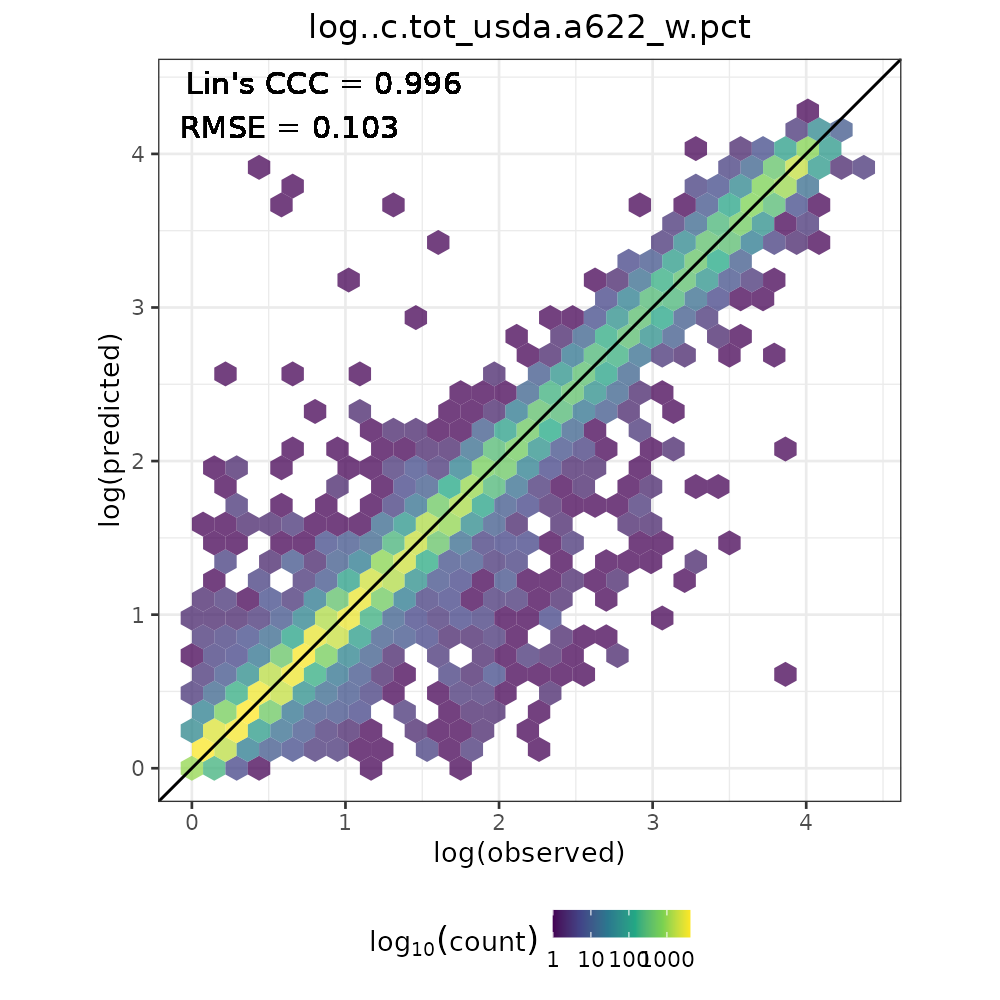
\includegraphics[width=0.7\textwidth,height=\textheight]{index_files/mediabag/valplot_mir_cubist_o.png}

}

\caption{Validation scatterplot for
\texttt{log..c.tot\_usda.a622\_w.pct} using
\texttt{mir\_cubist\_ossl\_na\_v1.2}.}

\end{figure}%

\section{Uncertainty and representation
flag}\label{uncertainty-and-representation-flag}

The cross-validated predictions were used to estimate the unbiased
absolute error, which was employed to calibrate uncertainty estimaton
models via
\href{https://en.wikipedia.org/wiki/Conformal_prediction}{conformal
prediction}.The conformal prediction is built upon past experience,
i.e.~the error model is calibrated using the same fine-tuned structure
of the respective response model.

Non-conformity scores of the calibration set were estimated from the
predicted error with a defined confidence level of 68\% to approximate
one standard deviation. The prediction interval (PI) can be derived by
estimating the response and error values corrected by the non-conformity
score of the calibration set {[}25,26{]}.

The main advantage of conformal prediction is that the intervals are
always covered, i.e.~a confidence of 68\% means that the predicted
interval regions may contain the observed value in at least 68\% of the
cases. Another big advantage of conformal prediction is that it is model
agnostic and we get rid of resampling mechanisms such as bootstrapping
or Monte Carlo simulation which significantly requires a huge
computation time for large sample sizes.

The representation flag was built using the PCA model employed for
compression {[}19,20{]}. Considering that only the first 120 PCs are
used to decompose spectra for modeling fitting, the remaining variation
from farther components are residual. The difference between the
original spectra and back-transformed with the first 120 PCs made
possible the calculation of the Q-statistics (sum of squared residual
across the spectrum). The Q statistic of new spectra are compared
against a Q critical value estimated from the calibration set with a
99\% confidence level.

\section{Local run of the OSSL
models}\label{local-run-of-the-ossl-models}

Please follow the instructions provided in the
\href{https://github.com/soilspectroscopy/ossl-nix}{\textbf{ossl-nix}}
GitHub repository for a full reproducible and local execution of the
OSSL models.

\bookmarksetup{startatroot}

\chapter{Web services}\label{sec-web-services}

\section{\texorpdfstring{\href{https://explorer.soilspectroscopy.org/}{OSSL
Explorer}}{OSSL Explorer}}\label{ossl-explorer}

The \href{https://explorer.soilspectroscopy.org/}{OSSL Explorer} is a
web platform where a user can explore the OSSL database. You can use it
to subset and explore the database based on geographical filters
(`Geography' tab) or on the range of soil properties (`Soil properties'
tab).

Once applied a selection, you can download the data by clicking on the
bottom right option `Download now'. If you want to restart the filters,
click `Clear selection'. For accessing the full database by other means
(programmatically) or just download it as \texttt{csv} or \texttt{qs}
format, please check the instructions at
\textbf{\href{https://soilspectroscopy.github.io/ossl-manual/ossl-database-access.html}{OSSL
database access}} section..

\begin{figure}[H]

{\centering \includegraphics[width=1\textwidth,height=\textheight]{img/explorer1.png}

}

\caption{OSSL Explorer initial page that allows filtering OSSL samples
based on geographical distribution.}

\end{figure}%

\begin{figure}[H]

{\centering \includegraphics[width=1\textwidth,height=\textheight]{img/explorer2.png}

}

\caption{OSSL Explorer page that allows filtering OSSL samples based on
range of soil properties.}

\end{figure}%

\section{\texorpdfstring{\href{https://engine.soilspectroscopy.org/}{OSSL
Engine}}{OSSL Engine}}\label{ossl-engine}

The \href{https://engine.soilspectroscopy.org/}{OSSL Engine} is a web
platform where a user can upload spectra from the \textbf{VisNIR
(400-2500 nm), NIR (1350-2550 nm), or MIR (600-4000 cm-1) ranges} and
get predictions back with uncertainty estimation and representativeness
flag.

The modeling framework, cross-validation performance metrics, and
further information can be found at
\textbf{\href{https://soilspectroscopy.github.io/ossl-manual/ossl-prediction-models.html}{OSSL
prediction models}} section.

Please, check some
\textbf{\href{https://github.com/soilspectroscopy/ossl-manual/tree/main/sample-data}{example
datasets}} for formatting your spectra to the file specifications. You
can upload either \texttt{csv}, \texttt{asd} or opus (\texttt{.0})
files.

\begin{tcolorbox}[enhanced jigsaw, title=\textcolor{quarto-callout-tip-color}{\faLightbulb}\hspace{0.5em}{Tip}, rightrule=.15mm, coltitle=black, opacityback=0, bottomrule=.15mm, colframe=quarto-callout-tip-color-frame, breakable, arc=.35mm, titlerule=0mm, toptitle=1mm, left=2mm, colback=white, toprule=.15mm, leftrule=.75mm, bottomtitle=1mm, opacitybacktitle=0.6, colbacktitle=quarto-callout-tip-color!10!white]

We recommend using the OSSL model type for getting predictions. KSSL
models are recommended when the spectra to be predicted have the same
instrument manufacturer/model as the KSSL library and the samples to be
predicted are well represented by the range of soil properties of
interest.

\end{tcolorbox}

\begin{figure}[H]

{\centering \includegraphics[width=1\textwidth,height=\textheight]{img/engine1.png}

}

\caption{OSSL Engine initial page for uploading data, confirming
spectra, and selecting model type.}

\end{figure}%

\begin{figure}[H]

{\centering \includegraphics[width=1\textwidth,height=\textheight]{img/engine2.png}

}

\caption{OSSL Engine page with the outputs from model predictions,
including response, uncertainty interval, and trustworthiness flag.}

\end{figure}%

\section{\texorpdfstring{\href{https://api.soilspectroscopy.org/__docs__/\#/}{OSSL
API}}{OSSL API}}\label{ossl-api}

The \href{https://api.soilspectroscopy.org/__docs__/\#/}{OSSL API}
(Application Programming Interface) is experimental and available to
construct customized requests to fetch data, models, and generate
predictions. The outputs of predictions can be obtained as
\href{https://www.json.org/json-en.html}{JSON} or \texttt{CSV} files.

The OSSL API is at the moment based on the
\href{https://www.rplumber.io/}{plumber R package} and is
\textbf{provided for testing purposes only}. Users can make predictions
with the pre-trained models for 20 spectra per request.

\begin{figure}[H]

{\centering \includegraphics[width=1\textwidth,height=\textheight]{img/preview_ossl_api_swagger.png}

}

\caption{OSSL API is available for testing.}

\end{figure}%

\bookmarksetup{startatroot}

\chapter{Hands-on tutorial}\label{sec-tutorial}

After a series of events in 2023, which included a training workshop on
\href{https://soilspectroscopy.github.io/soilspec-workshop/}{\textbf{Predictive
Soil Spectroscopy}} at the ACS International Meeting 2023 in St Louis -
MO, USA, we made available a hands-on tutorial where we walk-through the
reader on processing and predictive modeling steps that are currently
employed in the OSSL. Common concepts and analysis are also introduced.

\href{https://soilspectroscopy.github.io/soilspec-workshop/}{\includegraphics[width=1\textwidth,height=\textheight]{img/tutorial.png}}

In this tutorial, you will find information on why soil spectroscopy
should be a fit-for-purpose technology, why good predictions flow from
good data, and what are the best practices for model building.

Further on, we walk the reader through examples of data import,
preparation, visualization, spectra resampling, preprocessing, and
compression.

Lastly, we conclude the guide with an introduction the the MLR3 modeling
framework and basic Chemometrics, exploring aspects of data splitting
and resampling, model optimization, benchmarking, and uncertainty
estimation via conformal prediction.

We hope that this tutorial gives a good overview of predictive soil
spectroscopy and helps people explore new ideas.

\bookmarksetup{startatroot}

\chapter{Scientific publications}\label{sec-publications}

Please find bellow all scientific publications that our team or
collaborators have published right before or during the project
timeline. We will keep listing all soil spectroscopy works derived from
the SS4GG activities and extended collaborations:

\begin{itemize}
\item
  Sanderman, J., Partida, C., Safanelli, J. L., Shepherd, K., Ge, Y.,
  Mitu, S. M., \& Ferguson, R. (2025). Application of a Handheld Near
  Infrared Spectrophotometer to Farm‐Scale Soil Carbon Monitoring. In
  European Journal of Soil Science (Vol. 76, Issue 1). Wiley.
  \url{https://doi.org/10.1111/ejss.70053}
\item
  Safanelli, J. L., Hengl, T., Parente, L. L., Minarik, R., Bloom, D.
  E., Todd-Brown, K., Gholizadeh, A., Mendes, W. de S., \& Sanderman, J.
  (2025). Open Soil Spectral Library (OSSL): Building reproducible soil
  calibration models through open development and community engagement.
  In B. Das (Ed.), PLOS ONE (Vol. 20, Issue 1, p.~e0296545). Public
  Library of Science (PLoS).
  \url{https://doi.org/10.1371/journal.pone.0296545}
\item
  Partida, C., Safanelli, J. L., Mitu, S. M., Murad, M. O. F., Ge, Y.,
  Ferguson, R., Shepherd, K., \& Sanderman, J. (2025). Building a
  near-infrared (NIR) soil spectral dataset and predictive machine
  learning models using a handheld NIR spectrophotometer. In Data in
  Brief (Vol. 58, p.~111229). Elsevier BV.
  \url{https://doi.org/10.1016/j.dib.2024.111229}
\item
  Mitu, S. M., Smith, C., Sanderman, J., Ferguson, R. R., Shepherd, K.,
  \& Ge, Y. (2024). Evaluating consistency across multiple NeoSpectra
  (compact Fourier transform near‐infrared) spectrometers for estimating
  common soil properties. In Soil Science Society of America Journal
  (Vol. 88, Issue 4, pp.~1324--1339). Wiley.
  \url{https://doi.org/10.1002/saj2.20678}
\item
  Safanelli, J. L., Sanderman, J., Bloom, D., Todd-Brown, K., Parente,
  L. L., Hengl, T., Adam, S., Albinet, F., Ben-Dor, E., Boot, C. M.,
  Bridson, J. H., Chabrillat, S., Deiss, L., Demattê, J. A. M., Scott
  Demyan, M., Dercon, G., Doetterl, S., van Egmond, F., Ferguson, R.,
  \ldots{} Żelazny, W. R. (2023). An interlaboratory comparison of
  mid-infrared spectra acquisition: Instruments and procedures matter.
  In Geoderma (Vol. 440, p.~116724). Elsevier BV.
  \url{https://doi.org/10.1016/j.geoderma.2023.116724}
\item
  Hong, Y., Sanderman, J., Hengl, T., Chen, S., Wang, N., Xue, J., Zhuo,
  Z., Peng, J., Li, S., Chen, Y., Liu, Y., Mouazen, A. M., \& Shi, Z.
  (2024). Potential of globally distributed topsoil mid-infrared
  spectral library for organic carbon estimation. In CATENA (Vol. 235,
  p.~107628). Elsevier BV.
  \url{https://doi.org/10.1016/j.catena.2023.107628}
\item
  Sanderman, J., Smith, C., Safanelli, J. L., Morgan, C. L. S.,
  Ackerson, J., Looker, N., Mathers, C., Keating, R., \& Kumar, A. A.
  (2023). Diffuse reflectance mid-infrared spectroscopy is viable
  without fine milling. In Soil Security (Vol. 13, p.~100104). Elsevier
  BV. \url{https://doi.org/10.1016/j.soisec.2023.100104}
\item
  Sanderman, J., Gholizadeh, A., Pittaki‐Chrysodonta, Z., Huang, J.,
  Safanelli, J. L., \& Ferguson, R. (2023). Transferability of a large
  mid‐infrared soil spectral library between two Fourier‐transform
  infrared spectrometers. In Soil Science Society of America Journal
  (Vol. 87, Issue 3, pp.~586--599). Wiley.
  \url{https://doi.org/10.1002/saj2.20513}
\item
  Shepherd, K. D., Ferguson, R., Hoover, D., van Egmond, F., Sanderman,
  J., \& Ge, Y. (2022). A global soil spectral calibration library and
  estimation service. In Soil Security (Vol. 7, p.~100061). Elsevier BV.
  \url{https://doi.org/10.1016/j.soisec.2022.100061}
\item
  Sanderman, J., Savage, K., Dangal, S. R. S., Duran, G., Rivard, C.,
  Cavigelli, M. A., Gollany, H. T., Jin, V. L., Liebig, M. A., Omondi,
  E. C., Rui, Y., \& Stewart, C. (2021). Can Agricultural Management
  Induced Changes in Soil Organic Carbon Be Detected Using Mid-Infrared
  Spectroscopy? In Remote Sensing (Vol. 13, Issue 12, p.~2265). MDPI AG.
  \url{https://doi.org/10.3390/rs13122265}
\item
  Gholizadeh, A., Neumann, C., Chabrillat, S., van Wesemael, B.,
  Castaldi, F., Borůvka, L., Sanderman, J., Klement, A., \& Hohmann, C.
  (2021). Soil organic carbon estimation using VNIR--SWIR spectroscopy:
  The effect of multiple sensors and scanning conditions. In Soil and
  Tillage Research (Vol. 211, p.~105017). Elsevier BV.
  \url{https://doi.org/10.1016/j.still.2021.105017}
\item
  Pittaki‐Chrysodonta, Z., Hartemink, A. E., Sanderman, J., Ge, Y., \&
  Huang, J. (2021). Evaluating three calibration transfer methods for
  predictions of soil properties using mid‐infrared spectroscopy. In
  Soil Science Society of America Journal (Vol. 85, Issue 3,
  pp.~501--519). Wiley. \url{https://doi.org/10.1002/saj2.20225}
\item
  Dangal, S. R. S., \& Sanderman, J. (2020). Is Standardization
  Necessary for Sharing of a Large Mid-Infrared Soil Spectral Library?
  In Sensors (Vol. 20, Issue 23, p.~6729). MDPI AG.
  \url{https://doi.org/10.3390/s20236729}
\item
  Sanderman, J., Savage, K., \& Dangal, S. R. S. (2020). Mid‐infrared
  spectroscopy for prediction of soil health indicators in the United
  States. In Soil Science Society of America Journal (Vol. 84, Issue 1,
  pp.~251--261). Wiley. \url{https://doi.org/10.1002/saj2.20009}
\item
  Dangal, S. R. S., Sanderman, J., Wills, S., \& Ramirez-Lopez, L.
  (2019). Accurate and Precise Prediction of Soil Properties from a
  Large Mid-Infrared Spectral Library. In Soil Systems (Vol. 3, Issue 1,
  p.~11). MDPI AG. \url{https://doi.org/10.3390/soilsystems3010011}
\end{itemize}

\bookmarksetup{startatroot}

\chapter*{References}\label{references}
\addcontentsline{toc}{chapter}{References}

\markboth{References}{References}

\phantomsection\label{refs}
\begin{CSLReferences}{0}{1}
\bibitem[\citeproctext]{ref-wijewardane2018predicting}
\CSLLeftMargin{1. }%
\CSLRightInline{Wijewardane NK, Ge Y, Wills S, Libohova Z. {Predicting
physical and chemical properties of US soils with a mid-infrared
reflectance spectral library}. Soil Science Society of America Journal.
2018;82: 722--731.
doi:\href{https://doi.org/10.2136/sssaj2017.10.0361}{10.2136/sssaj2017.10.0361}}

\bibitem[\citeproctext]{ref-Wijewardane2016}
\CSLLeftMargin{2. }%
\CSLRightInline{Wijewardane NK, Ge Y, Wills S, Loecke T. Prediction of
soil carbon in the conterminous united states: Visible and near infrared
reflectance spectroscopy analysis of the rapid carbon assessment
project. Soil Science Society of America Journal. 2016;80: 973--982.
doi:\href{https://doi.org/10.2136/sssaj2016.02.0052}{10.2136/sssaj2016.02.0052}}

\bibitem[\citeproctext]{ref-aitkenhead2018exploring}
\CSLLeftMargin{3. }%
\CSLRightInline{Aitkenhead MJ, Black HI. {Exploring the impact of
different input data types on soil variable estimation using the
ICRAF-ISRIC global soil spectral database}. Applied spectroscopy.
2018;72: 188--198.
doi:\href{https://doi.org/10.1177/0003702817739013}{10.1177/0003702817739013}}

\bibitem[\citeproctext]{ref-Vagen_2020}
\CSLLeftMargin{4. }%
\CSLRightInline{Vagen T-G, Winowiecki LA, Desta L, Tondoh EJ, Weullow E,
Shepherd K, et al. {Mid-Infrared Spectra (MIRS) from ICRAF Soil and
Plant Spectroscopy Laboratory: Africa Soil Information Service (AfSIS)
Phase I 2009-2013}. World Agroforestry - Research Data Repository; 2020.
doi:\href{https://doi.org/10.34725/DVN/QXCWP1}{10.34725/DVN/QXCWP1}}

\bibitem[\citeproctext]{ref-orgiazzi2018lucas}
\CSLLeftMargin{5. }%
\CSLRightInline{Orgiazzi A, Ballabio C, Panagos P, Jones A,
Fernández-Ugalde O. {LUCAS Soil, the largest expandable soil dataset for
Europe: a review}. European Journal of Soil Science. 2018;69: 140--153.
doi:\href{https://doi.org/10.1111/ejss.12499}{10.1111/ejss.12499}}

\bibitem[\citeproctext]{ref-Summerauer2021}
\CSLLeftMargin{6. }%
\CSLRightInline{Summerauer L, Baumann P, Ramirez-Lopez L, Barthel M,
Bauters M, Bukombe B, et al. The central african soil spectral library:
A new soil infrared repository and a geographical prediction analysis.
SOIL. 2021;7: 693--715.
doi:\href{https://doi.org/10.5194/soil-7-693-2021}{10.5194/soil-7-693-2021}}

\bibitem[\citeproctext]{ref-Schiedung2022}
\CSLLeftMargin{7. }%
\CSLRightInline{Schiedung M, Bellè S-L, Malhotra A, Abiven S. Organic
carbon stocks, quality and prediction in permafrost-affected forest
soils in north canada. {CATENA}. 2022;213: 106194.
doi:\href{https://doi.org/10.1016/j.catena.2022.106194}{10.1016/j.catena.2022.106194}}

\bibitem[\citeproctext]{ref-Garrett2022}
\CSLLeftMargin{8. }%
\CSLRightInline{Garrett LG, Sanderman J, Palmer DJ, Dean F, Patel S,
Bridson JH, et al. Mid-infrared spectroscopy for planted forest soil and
foliage nutrition predictions, new zealand case study. Trees, Forests
and People. 2022;8: 100280.
doi:\href{https://doi.org/10.1016/j.tfp.2022.100280}{10.1016/j.tfp.2022.100280}}

\bibitem[\citeproctext]{ref-Jovi2019}
\CSLLeftMargin{9. }%
\CSLRightInline{Jović B, Ćirić V, Kovačević M, Šeremešić S, Kordić B.
Empirical equation for preliminary assessment of soil texture.
Spectrochimica Acta Part A: Molecular and Biomolecular Spectroscopy.
2019;206: 506--511.
doi:\href{https://doi.org/10.1016/j.saa.2018.08.039}{10.1016/j.saa.2018.08.039}}

\bibitem[\citeproctext]{ref-Safanelli2025}
\CSLLeftMargin{10. }%
\CSLRightInline{Safanelli JL, Hengl T, Parente LL, Minarik R, Bloom DE,
Todd-Brown K, et al. Open soil spectral library ({OSSL)}: Building
reproducible soil calibration models through open development and
community engagement. PLoS One. 2025;20: e0296545.
doi:\href{https://doi.org/10.1371/journal.pone.0296545}{10.1371/journal.pone.0296545}}

\bibitem[\citeproctext]{ref-BenedettiEgmond2021}
\CSLLeftMargin{11. }%
\CSLRightInline{Benedetti F, van Egmond F. {Global Soil Spectroscopy
Assessment. Spectral soil data --- Needs and capacities}. Rome, Italy:
FAO; 2021. p. 42.
doi:\href{https://doi.org/10.4060/cb6265en}{10.4060/cb6265en}}

\bibitem[\citeproctext]{ref-Safanelli2023}
\CSLLeftMargin{12. }%
\CSLRightInline{Safanelli JL, Sanderman J, Bloom D, Todd-Brown K,
Parente LL, Hengl T, et al. An interlaboratory comparison of
mid-infrared spectra acquisition: Instruments and procedures matter.
Geoderma. 2023;440: 116724.
doi:\href{https://doi.org/10.1016/j.geoderma.2023.116724}{10.1016/j.geoderma.2023.116724}}

\bibitem[\citeproctext]{ref-Partida2025}
\CSLLeftMargin{13. }%
\CSLRightInline{Partida C, Safanelli JL, Mitu SM, Murad MOF, Ge Y,
Ferguson R, et al. Building a near-infrared ({NIR}) soil spectral
dataset and predictive machine learning models using a handheld {NIR}
spectrophotometer. Data Brief. 2025;58: 111229.
doi:\href{https://doi.org/10.1016/j.dib.2024.111229}{10.1016/j.dib.2024.111229}}

\bibitem[\citeproctext]{ref-Mitu2024}
\CSLLeftMargin{14. }%
\CSLRightInline{Mitu SM, Smith C, Sanderman J, Ferguson RR, Shepherd K,
Ge Y. Evaluating consistency across multiple {NeoSpectra} (compact
fourier transform near‐infrared) spectrometers for estimating common
soil properties. Soil Sci Soc Am J. 2024;88: 1324--1339.
doi:\href{https://doi.org/10.1002/saj2.20678}{10.1002/saj2.20678}}

\bibitem[\citeproctext]{ref-mlr3}
\CSLLeftMargin{15. }%
\CSLRightInline{Lang M, Binder M, Richter J, Schratz P, Pfisterer F,
Coors S, et al. {mlr3}: A modern object-oriented machine learning
framework in {R}. Journal of Open Source Software. 2019.
doi:\href{https://doi.org/10.21105/joss.01903}{10.21105/joss.01903}}

\bibitem[\citeproctext]{ref-quinlan1992learning}
\CSLLeftMargin{16. }%
\CSLRightInline{Quinlan J. Learning with continuous classes. Proc 5th
australian joint conference on artificial intelligence, tasmania, 1992.
1992. pp. 343--348. }

\bibitem[\citeproctext]{ref-quinlan1993combining}
\CSLLeftMargin{17. }%
\CSLRightInline{Quinlan J. Combining instance-based and model-based
learning. Proc Tenth int Conference on machine learning. 1993. pp.
236--243. }

\bibitem[\citeproctext]{ref-chang2001near}
\CSLLeftMargin{18. }%
\CSLRightInline{Chang C-W, Laird D, Mausbach MJ, Hurburgh Jr CR.
Near-infrared reflectance spectroscopy--principal components regression
analyses of soil properties. Soil Science Society of America Journal.
2001;65: 480.
doi:\href{https://doi.org/10.2136/sssaj2001.652480x}{10.2136/sssaj2001.652480x}}

\bibitem[\citeproctext]{ref-Jackson1979}
\CSLLeftMargin{19. }%
\CSLRightInline{Jackson JE, Mudholkar GS. Control procedures for
residuals associated with principal component analysis. Technometrics.
1979;21: 341--349.
doi:\href{https://doi.org/10.1080/00401706.1979.10489779}{10.1080/00401706.1979.10489779}}

\bibitem[\citeproctext]{ref-deSantana2023}
\CSLLeftMargin{20. }%
\CSLRightInline{Santana FB de, Hall RebeccaL, Lowe V, Browne MA, Grunsky
EC, Fitzsimons MM, et al. A systematic approach to predicting and
mapping soil particle size distribution from unknown samples using large
mid-infrared spectral libraries covering large-scale heterogeneous
areas. Geoderma. 2023;434: 116491.
doi:\href{https://doi.org/10.1016/j.geoderma.2023.116491}{10.1016/j.geoderma.2023.116491}}

\bibitem[\citeproctext]{ref-Barnes1989}
\CSLLeftMargin{21. }%
\CSLRightInline{Barnes RJ, Dhanoa MS, Lister SJ. Standard normal variate
transformation and de-trending of near-infrared diffuse reflectance
spectra. Applied Spectroscopy. 1989;43: 772--777.
doi:\href{https://doi.org/10.1366/0003702894202201}{10.1366/0003702894202201}}

\bibitem[\citeproctext]{ref-Yang2020}
\CSLLeftMargin{22. }%
\CSLRightInline{Yang L, Shami A. On hyperparameter optimization of
machine learning algorithms: Theory and practice. Neurocomputing.
2020;415: 295--316.
doi:\href{https://doi.org/10.1016/j.neucom.2020.07.061}{10.1016/j.neucom.2020.07.061}}

\bibitem[\citeproctext]{ref-Dangal2019}
\CSLLeftMargin{23. }%
\CSLRightInline{Dangal S, Sanderman J, Wills S, Ramirez-Lopez L.
Accurate and precise prediction of soil properties from a large
mid-infrared spectral library. Soil Systems. 2019;3: 11.
doi:\href{https://doi.org/10.3390/soilsystems3010011}{10.3390/soilsystems3010011}}

\bibitem[\citeproctext]{ref-malone2021soil}
\CSLLeftMargin{24. }%
\CSLRightInline{Wadoux AMJC, Malone B, McBratney AB, Fajardo M, Minasny
B. {Soil Spectral Inference with R: Analysing Digital Soil Spectra Using
the R Programming Environment}. Springer International Publishing; 2021.
}

\bibitem[\citeproctext]{ref-Norinder2014}
\CSLLeftMargin{25. }%
\CSLRightInline{Norinder U, Carlsson L, Boyer S, Eklund M. Introducing
conformal prediction in predictive modeling. A transparent and flexible
alternative to applicability domain determination. Journal of Chemical
Information and Modeling. 2014;54: 1596--1603.
doi:\href{https://doi.org/10.1021/ci5001168}{10.1021/ci5001168}}

\bibitem[\citeproctext]{ref-CortsCiriano2015}
\CSLLeftMargin{26. }%
\CSLRightInline{Cortés-Ciriano I, Westen GJP van, Bouvier G, Nilges M,
Overington JP, Bender A, et al. Improved large-scale prediction of
growth inhibition patterns using the {NCI}60 cancer cell line panel.
Bioinformatics. 2015;32: 85--95.
doi:\href{https://doi.org/10.1093/bioinformatics/btv529}{10.1093/bioinformatics/btv529}}

\end{CSLReferences}



\end{document}
